\documentclass[12pt]{article}
\usepackage[letterpaper, margin=1in]{geometry}
\usepackage[utf8]{inputenc}
%\usepackage{natbib}
\usepackage{hyperref}
\usepackage{graphicx}
%\usepackage{indentfirst}
\usepackage{float}
\usepackage{dirtytalk}
\usepackage{subcaption}
\usepackage{tikz}
\usepackage{siunitx}
\usepackage[T1]{fontenc}
\usepackage{booktabs}
\usepackage[autostyle]{csquotes}
\usepackage{amsmath}
\usepackage{indentfirst}
\usepackage{float}
\usepackage[square, numbers, comma, sort&compress]{natbib}
\usepackage[acronym]{glossaries}



\newacronym{D-A}{D-A}{Donor-Acceptor}
\newacronym{BHJs}{BHJs}{Bulk Heterojunctions}
\newacronym{BHJ}{BHJ}{Bulk Heterojunction}
\newacronym{bhj}{BHJ}{bulk heterojunctions}
\newacronym{bhjs}{BHJs}{bulk heterojunctions}
\newacronym{ET}{ET}{Electron Transfer}
\newacronym{et}{ET}{electron transfer}
\newacronym{CT}{CT}{Charge Transfer}
\newacronym{ct}{CT}{charge transfer}
\newacronym{Mos2}{MoS$_2$}{Molybdenum disulphide}
\newacronym{PTCDA}{PTCDA}{Perylenetetracarboxylic dianhydride}
\newacronym{PTCDI}{PTCDI}{perylenetetracarboxylic diimide}
\newacronym{MoS2/PTCDI}{MoS$_2$ / PTCDI}{MoS$_2$ / PTCDI}
\newacronym{MoS2/PTCDA}{MoS$_2$ / PTCDA}{MoS$_2$ / PTCDA}





\title{Maximizing photo-to-electrical conversion yield by entropy, electron delocalization and nanopatterns.}
\author{Kushal Rijal}
\date{July 8, 2022}
\begin{document}

\maketitle
\section*{\hfil Abstract\hfil}
The efficiency of organic photovoltaic devices (OPVs) had plateaued at $\sim$ 12 \% in the early 2010s until recently when it jumped to $\sim$ 18 \% after advances in the development of non-fullerene acceptors (NFAs) were made. This leap in efficiency can be attributed to the efficient exciton dissociation but the fundamental reason for it to occur in NFAs only is still not clear. In this proposed work, we plan to investigate this research problem by preparing different interfaces containing NFAs and studying the effects of entropy, electron delocalization, and nanopatterns on charge generation and transport, charge recombination, and charge separation using spectroscopic tools. By using ultraviolet photoemission spectroscopy (UPS) and time resolved pump-probe photoemission spectroscopy (TR-TPPE) experiments we can measure delocalization size, the dynamical evolution, and energy of excitonic states in organic molecules. Along with understanding the mechanism behind the surprising breakthrough in OPV efficiency, our results could help design other molecular an nanomaterials for efficient light harvesting applications, in the longer term. 

\section{Introduction}
The main task of any photovoltaic or photosensor device is to convert light into electricity. For commercial applications, these devices are usually desired to have high photo-to-electrical conversion yield along with low production costs. Solar cells based on organic semiconductors are starting to show power conversion efficiencies (PCEs $\sim$ 18$\%$) comparable to those of inorganic solar cells ( $\sim$ 33$\%$) \cite{hou2018organic,cariou2018iii}. A distinct advantage of organic solar cells (OSCs) over the inorganic solar cells comes from the fact that they can be low-cost, mechanically flexible, nontoxic, lightweight and solution-processable. A typical device structure of an organic solar cell is shown in Figure \ref{fig:1a}; the active material is sandwiched between two electrodes, electrode 1 and electrode 2. The active layer usually comprises at least two semiconducting materials, which are known as \lq{electron donors} (D) and \lq{electron acceptors} (A), and it is commonly designed in the form of bilayer heterojunctions (Figure \ref{fig:1b}) and \acrfull{bhjs} (Figure \ref{fig:1c}). OSCs require a D-A interface to dissociate tightly bound excitons into free charges.
 
\begin{figure}[H]
\centering
\subcaptionbox{\label{fig:1a}}{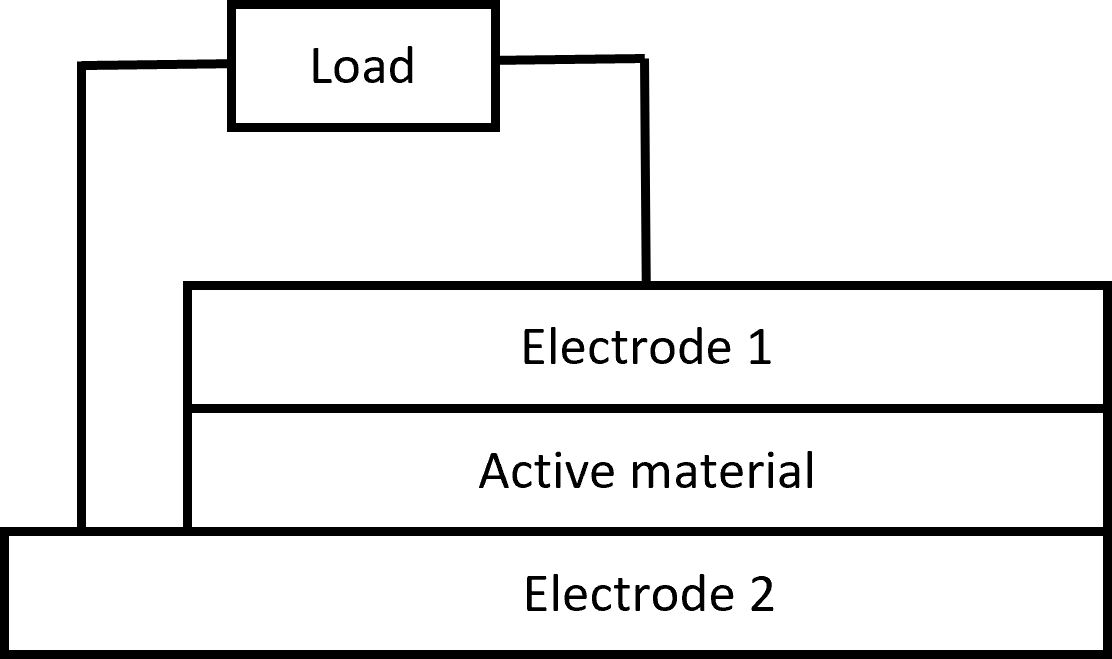
\includegraphics[width = 2.1 in]{device_structure.png}}
\subcaptionbox{\label{fig:1b}}{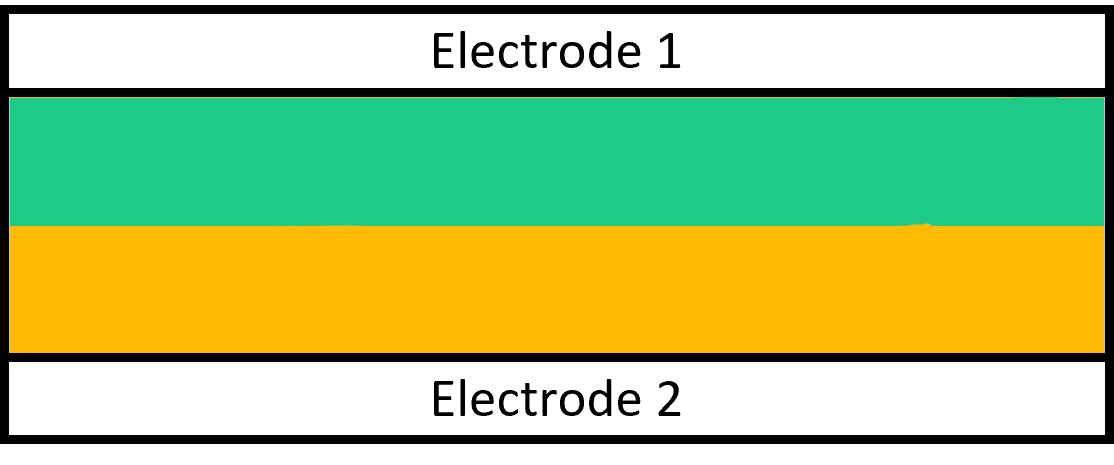
\includegraphics[width = 2.1 in]{bilayer_hetero.png}}
\subcaptionbox{\label{fig:1c}}{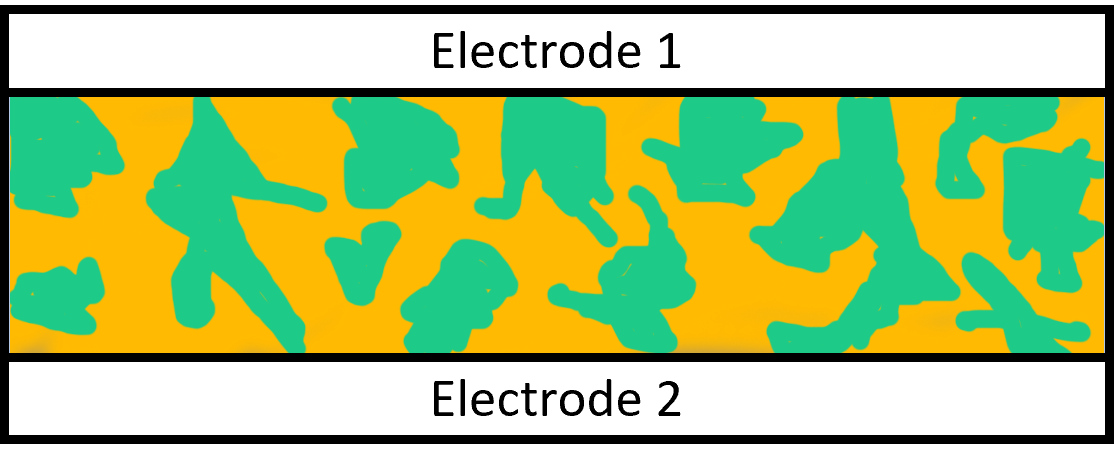
\includegraphics[width = 2.1 in]{bulk heterojunction.png}}
\caption{(a) Typical organic photovoltaic (OPV) device structure. Electrode 2 is transparent and allows light to reach the photoactive layer. (b) Bi-layer heterojunction. (c) Bulk heterojuction. The green and yellow color indicate the acceptor and donor molecules, respectively.}\label{fig:OPV devices}
\end{figure}



\subsection{Photogeneration mechanism}
\begin{figure}[H]
    \centering
    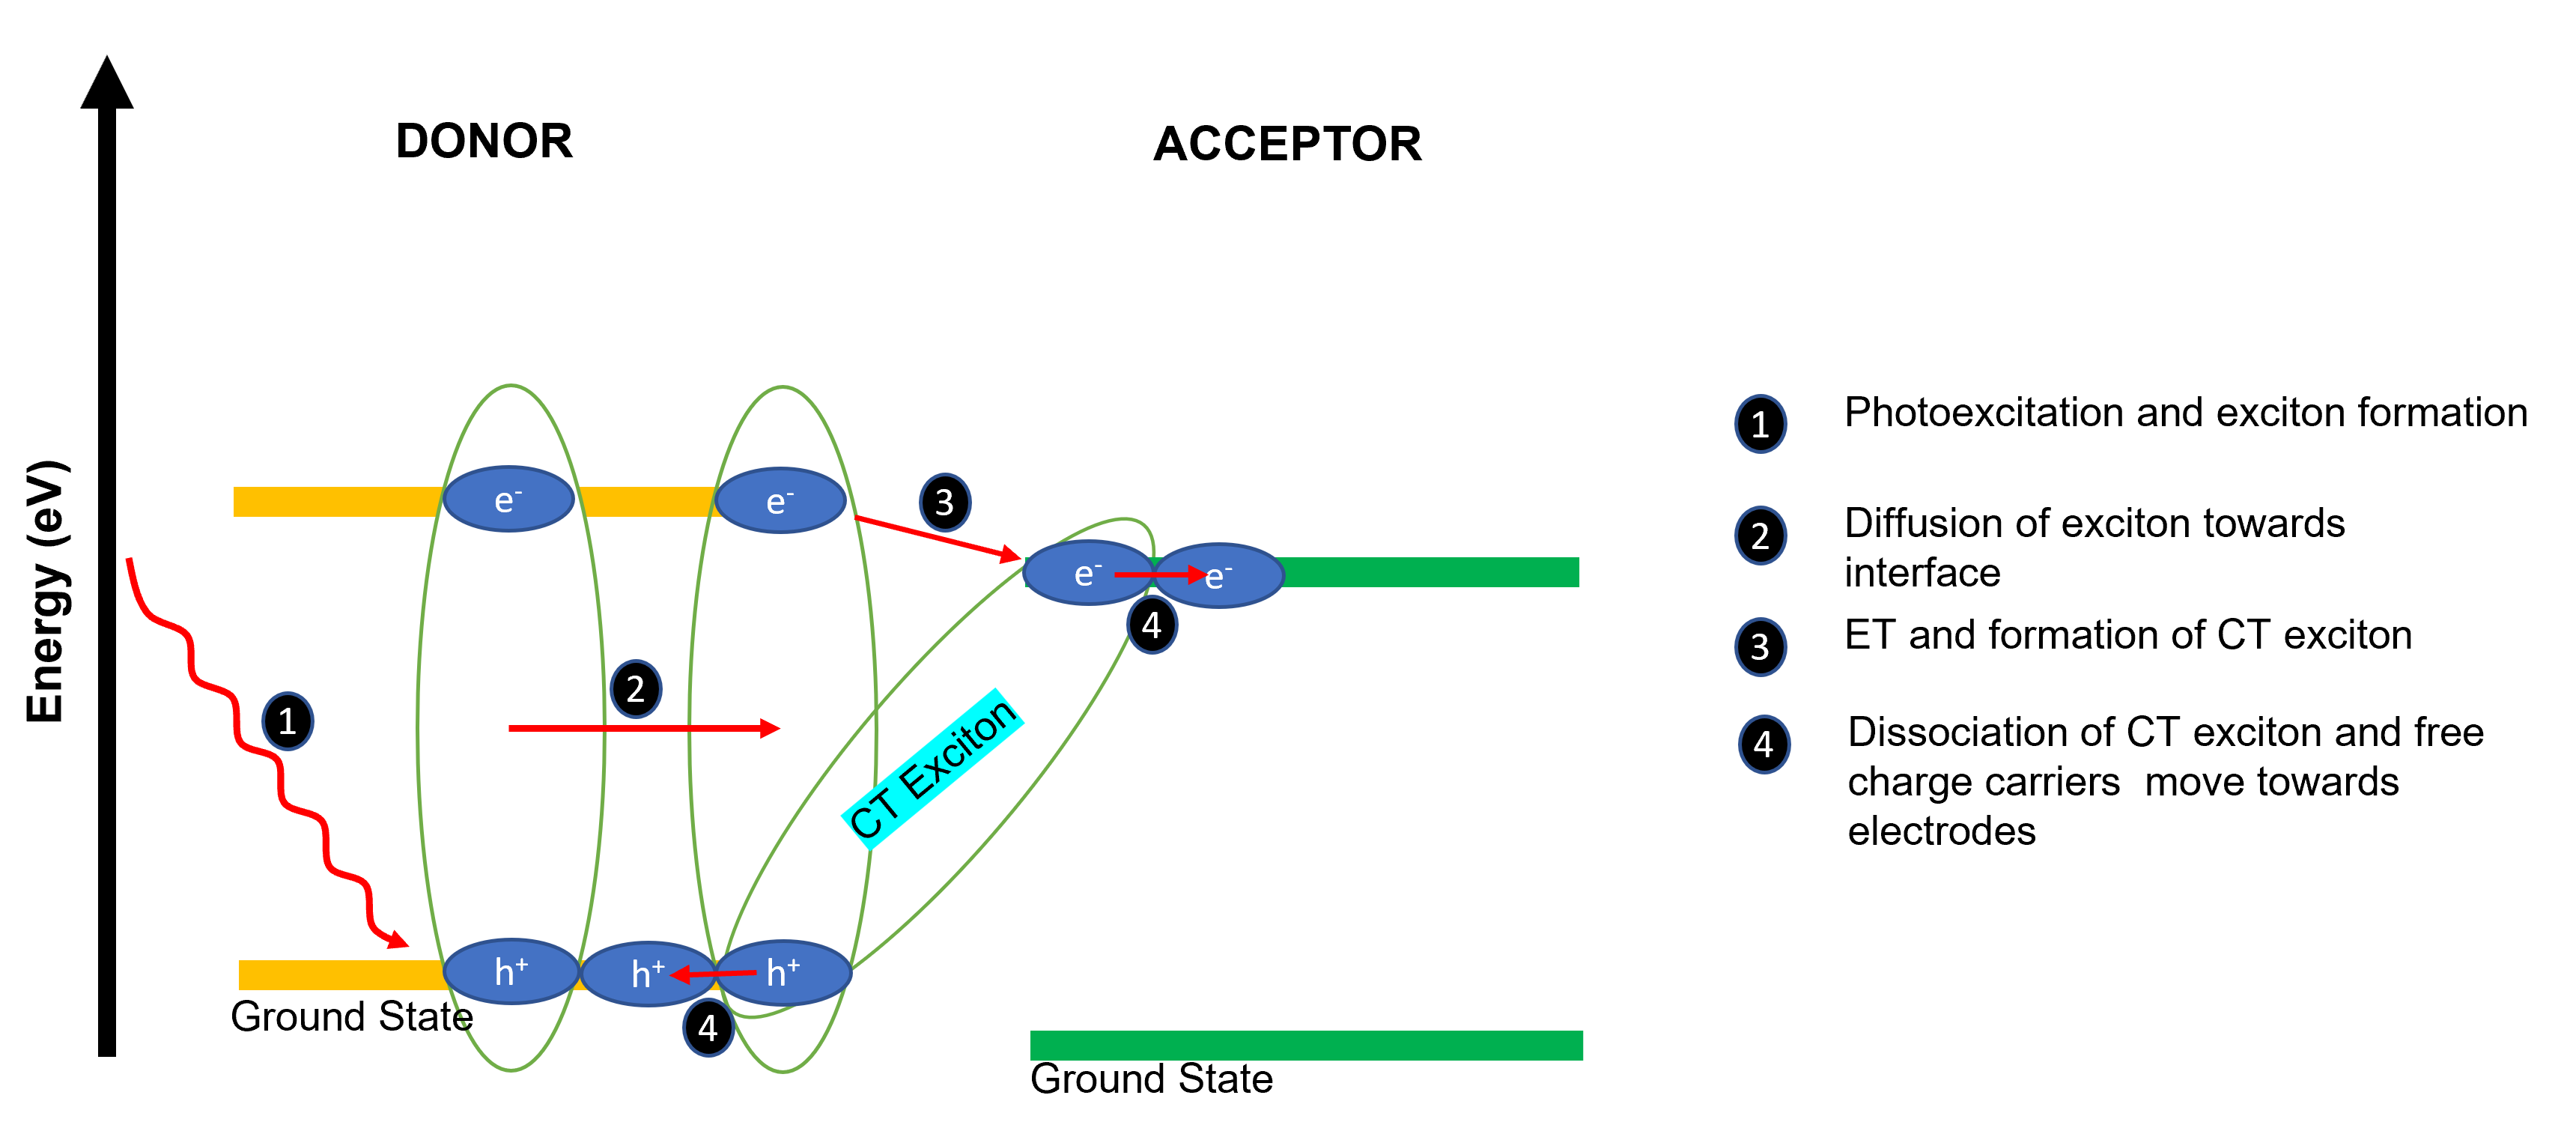
\includegraphics[scale = 0.6]{mechanism-CT.png}
    \caption{Mechanism of Photogeneration in heterojunctions with type-II band alignment}
    \label{fig:my_label}
\end{figure}
When photons are absorbed by the semiconductors, electrons in the ground state are excited to the bound excited states leaving the holes in the valence band. These electron-hole pairs, produced in donor molecules of the active layer, must diffuse towards the donor-acceptor (D-A) interface where electrons can be transferred to the acceptor molecules. The process of transfer of these electrons is facilitated by the type-II band alignment in the interface, where electrons relax onto the lower unoccupied energy level of the acceptor molecules. The offset ($E_{off}$) between the excited states of the donor and acceptor molecules provides the driving force necessary for electron transfer (ET) to occur. These excitons that reside at the D-A interface after the ET are known as charge transfer (CT) excitons. Generation of photocurrent is possible only if the bound charges in these CT excitons can dissociate before recombination. The excitonic state where CT excitons can dissociate and give free carriers is known as charge separation state (CS) state and the process is known as CS process. Finally, these free charges are collected at the electrodes, creating a potential difference and generating the electricity in the circuit.


\subsection{Exciton dissociation at the D-A interface}
The binding energies ($E_B$) of the excitons are given by the relation,
\begin{equation}
    E_B = \frac{e^2}{4\pi\epsilon_0\epsilon_rr}
\end{equation}
where, $e$, $r$, $\epsilon_0$, $\epsilon_r$ represent the charge of the electron, separation between electrons and holes, the permittivity of the free space and the dielectric constant of the material, respectively. The binding energy of the excitons can also be realized as the difference between the electronic band gap and the optical band gap of the material \cite{ugeda2014giant}. The electrical band gap is the amount of energy required to form an unbound electron-hole pairs, whereas the optical band gap is the minimum amount of energy required to form an exciton through optical excitation. In commonly studied semiconductors such as transitional metal dichalchogenides (TMDCs) and organic semiconductors due to weak dielectric screening, the binding energies are typically in the range of 0.1 eV to 1 eV, which is significantly higher than the thermal energy (25 meV) at room temperature \cite{knupfer2003exciton,pospischil2016optoelectronic}. For this reason, excitons do not dissociate readily to generate free electrons and holes. Furthermore, the electrons and holes in the CT excitons are in the close proximity of one another which results in a short lifetime making exciton dissociation a less probable event compared to the charge recombination, near the interface. However, in organic solar cells, there are reports of very high internal quantum efficiency (number of electron hole pairs generated per absorbed photon), with some approaching near 100\% for certain wavelengths \cite{park2009bulk}.


\begin{figure}[H]
\centering
\subcaptionbox{\label{fig:traditional}}{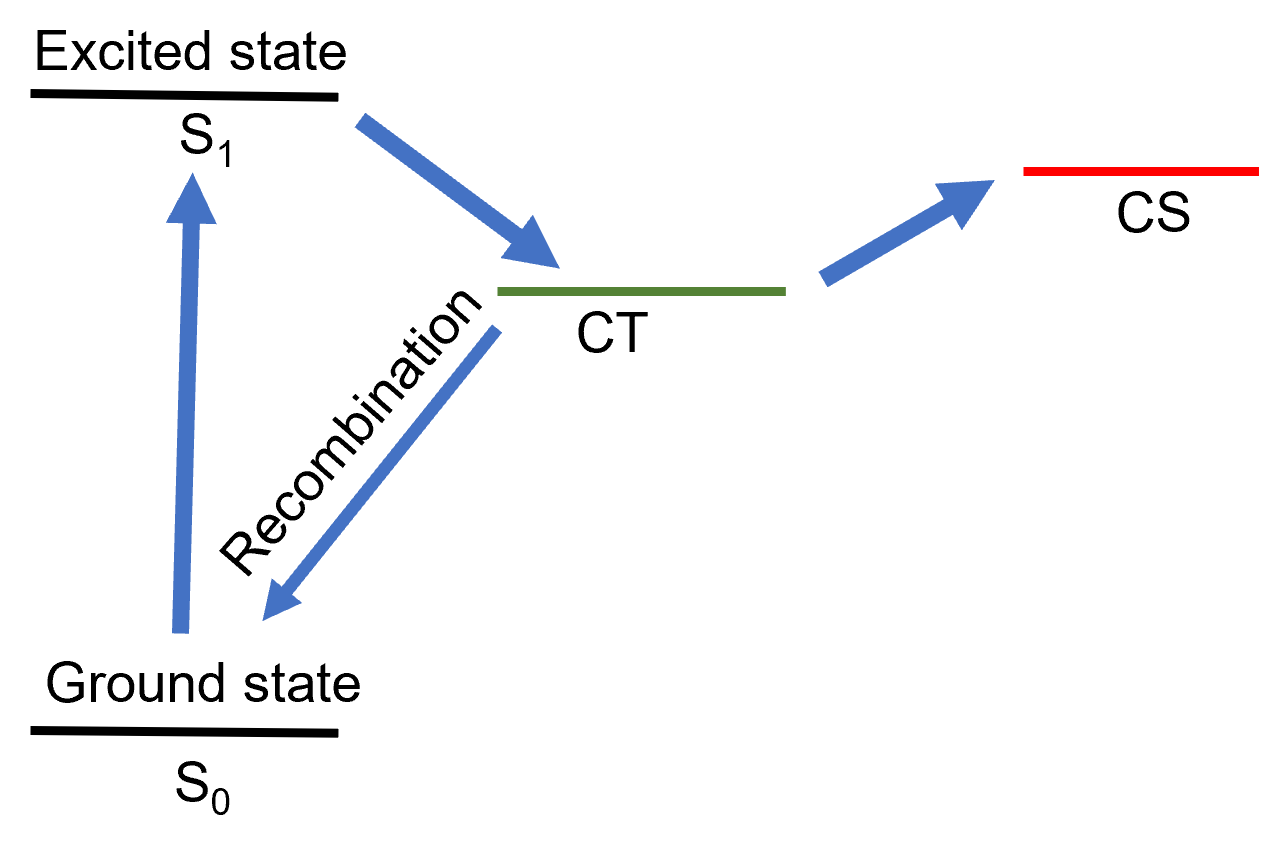
\includegraphics[scale = 0.82]{ColdCT.png}} \hspace{5pt}
\subcaptionbox{\label{fig:hot CT}}{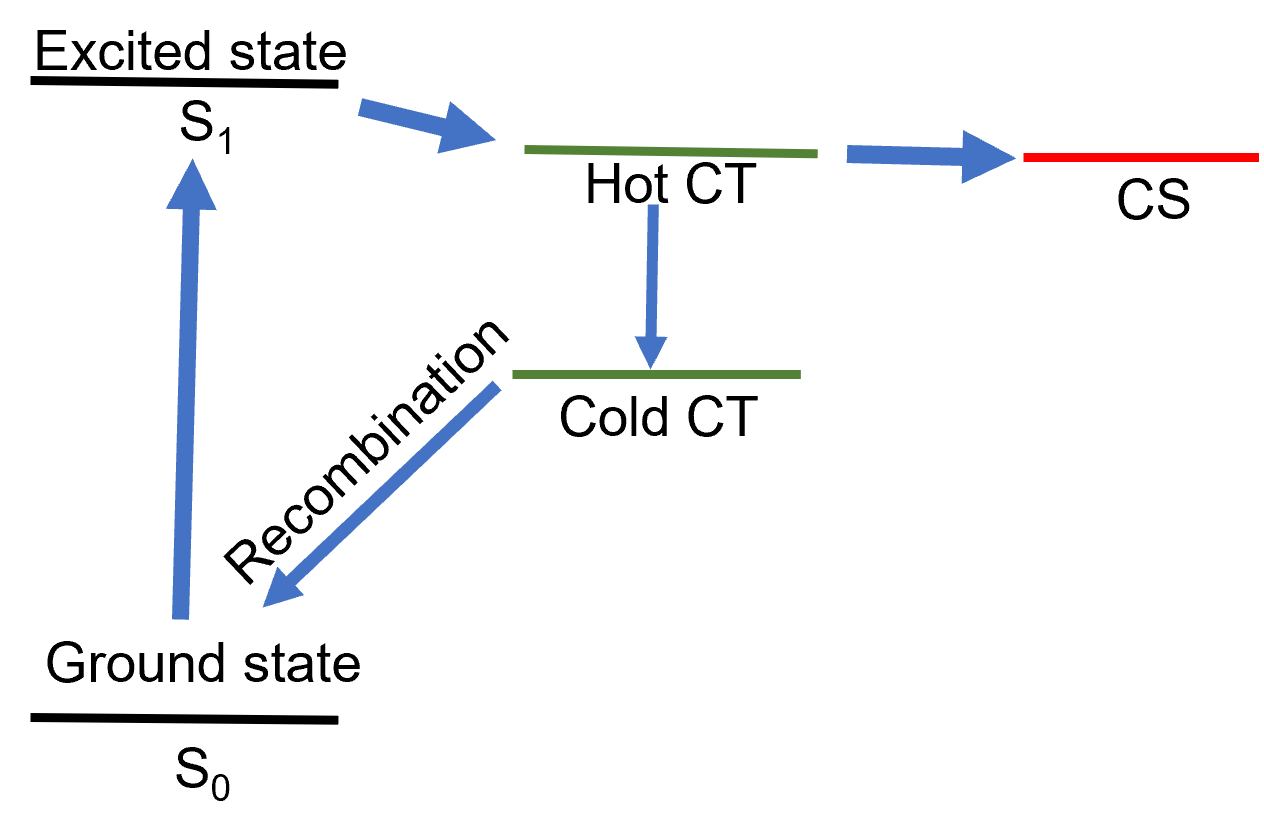
\includegraphics[scale = 0.82]{FA_hotct.png}}
\caption{Schematic diagram of the exciton dissociation mechanism at the D-A interface. (a) Traditional picture of the CS mechanism. (b) Hot CT picture of CS mechanism.}
\label{fig:hot and cold mechanism}
\end{figure}

To understand the mechanism behind such high efficiency, a hot process of charge transfer has been proposed where the excess energy ($E_{S_1} - E_{CT}$) originating from the band offset contributes to the dissociation of excitons in CT states \cite{clarke2010charge}. Here, $E_{S_1}$ and $E_{CT}$ represent the energies of the exciton in the S$_1$ and CT states, respectively. This model is supported by the fact that the number of free charge
carriers in the device increases as $\Delta E_{CT}$ gets larger but the rate of free carrier formation is temperature independent which means the charge separation is barrier-less \cite{ohkita2008charge,clarke2008free,pensack2009barrierless}. These 
 hot CT excitons are spatially-delocalized and have an energy close to that of the free electron-hole pair \cite{grancini2013hot,jailaubekov2013hot,gelinas2014ultrafast,savoie2014unequal}. Therefore, the whole CS process (from S$_1$ to the free e-h pair) can occur on an ultrafast (fs – ps) 
 timescale nearly iso-energetically by kinetically avoiding the lower-energy cold CT states \cite{grancini2013hot,jailaubekov2013hot,gelinas2014ultrafast,savoie2014unequal}. The dissociation of excitons can also occur from these cold CT states, but such processes are rather slow and temperature dependent \cite{bernede2008organic,gautam2016charge,athanasopoulos2017efficient,fazzi2017hot}.


\section{Motivation}
For applications such as organic photovoltaics (OPV), the separation of CT excitons is often associated with energy loss, resulting in the decrease in open-circuit voltage ($V_{oc}$) of the device and therefore the efficiency of the device \cite{yao2015quantifying,rand2007offset,liu2019engineering}. Mathematically, 
\begin{equation}
   V_{oc} = \frac{1}{e}( |E_{HOMO,D} - E_{LUMO,A}| - \Delta)
\end{equation}
 where, $E_{HOMO,D}$ , $E_{LUMO,A}$, and $\Delta$ refers to the highest occupied molecular orbital (HOMO) level of donor, lowest unoccupied molecular orbital (LUMO) level of acceptor and energy losses due to recombination, defects, interfacial energy disorder, etc. Although the excess energy provided by the band offset can promote charge separation and reduce losses due to recombination, it reduces the $V_{oc}$ and internal quantum efficiency of the device. This problem, unique to OPVs, has resulted in the efficiency of OPVs to be around 12\% for almost a decade since the early 2010s, which is smaller than the commercially available inorganic counterparts ($\sim$ 25\%).


\begin{figure}[H]
\centering
\subcaptionbox{\label{fig:NREL}}{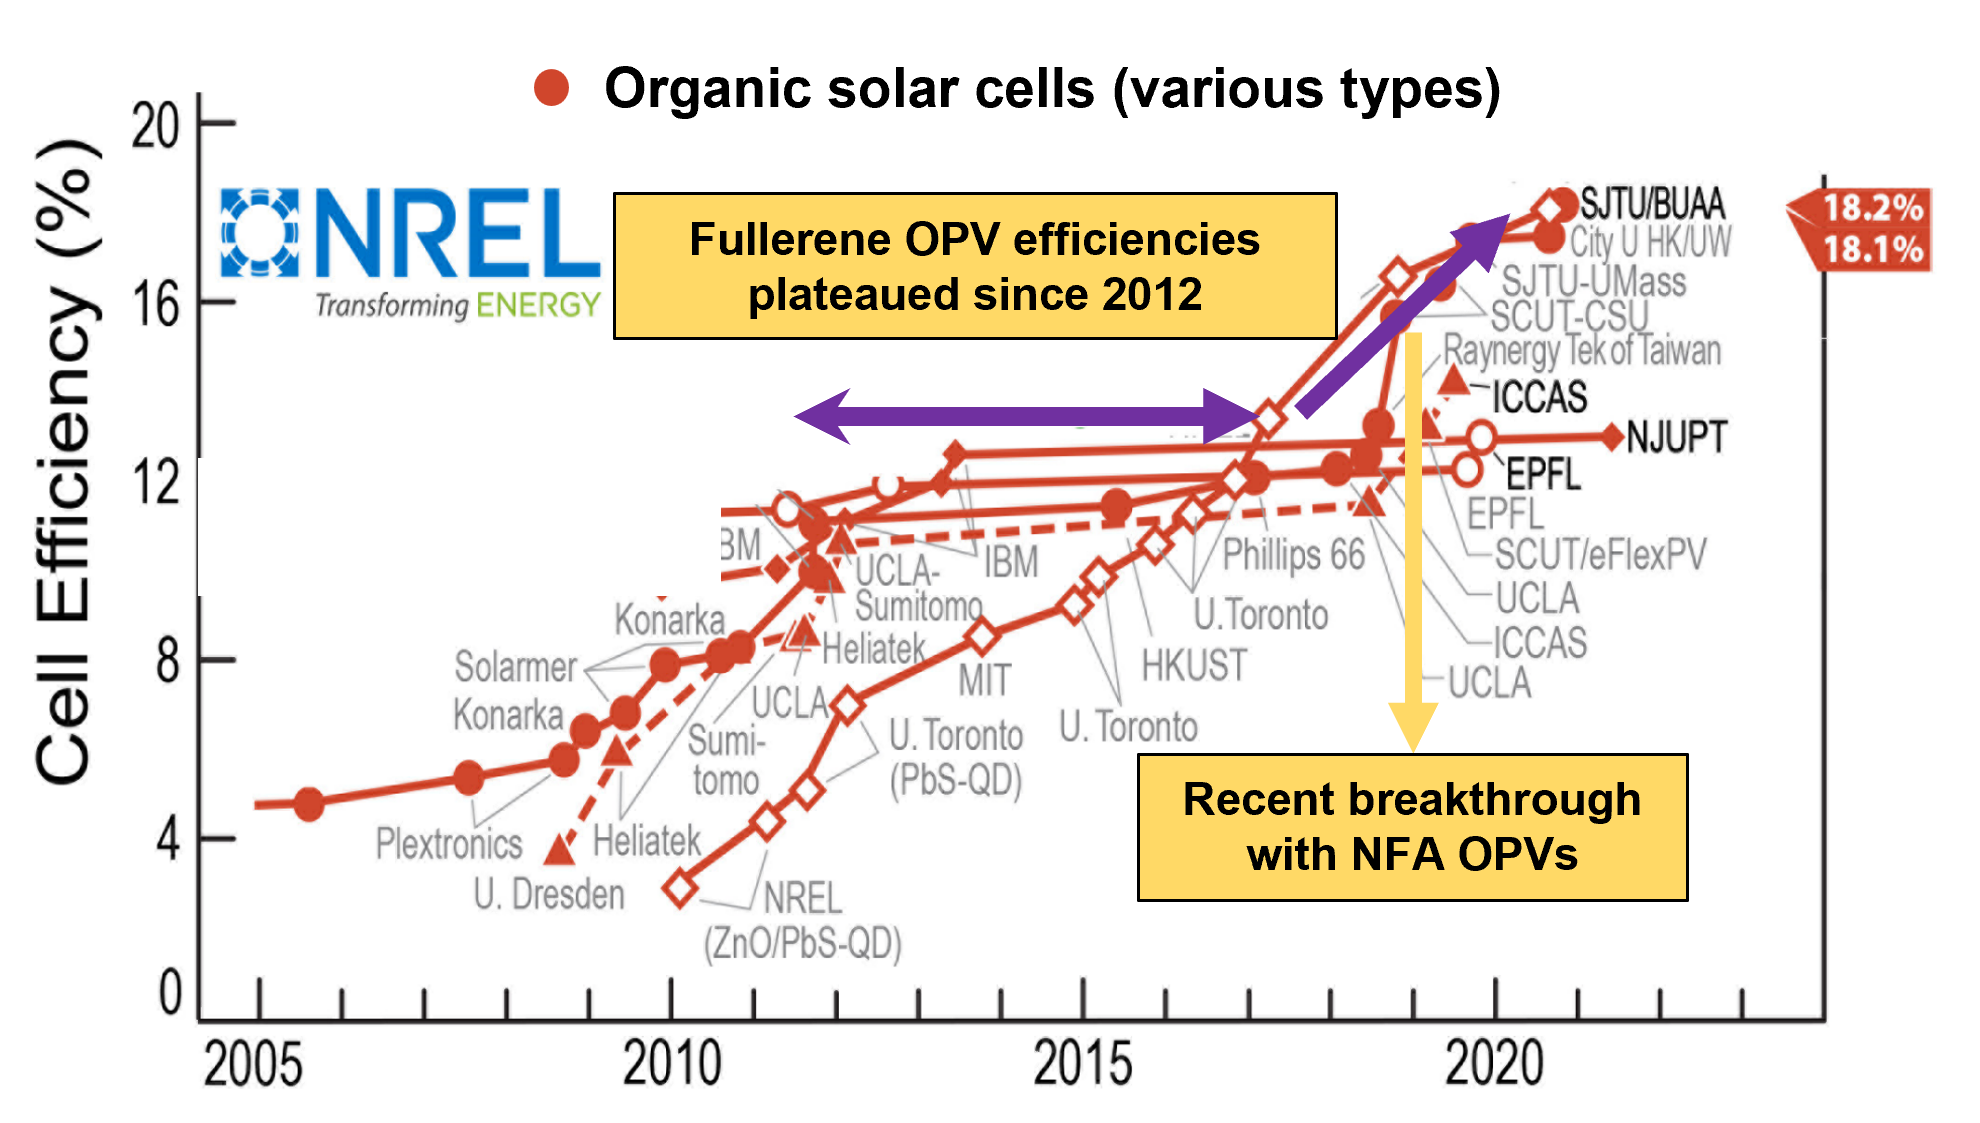
\includegraphics[scale = 0.6]{NREL.png}}
\subcaptionbox{\label{fig:NFAhot CT}}{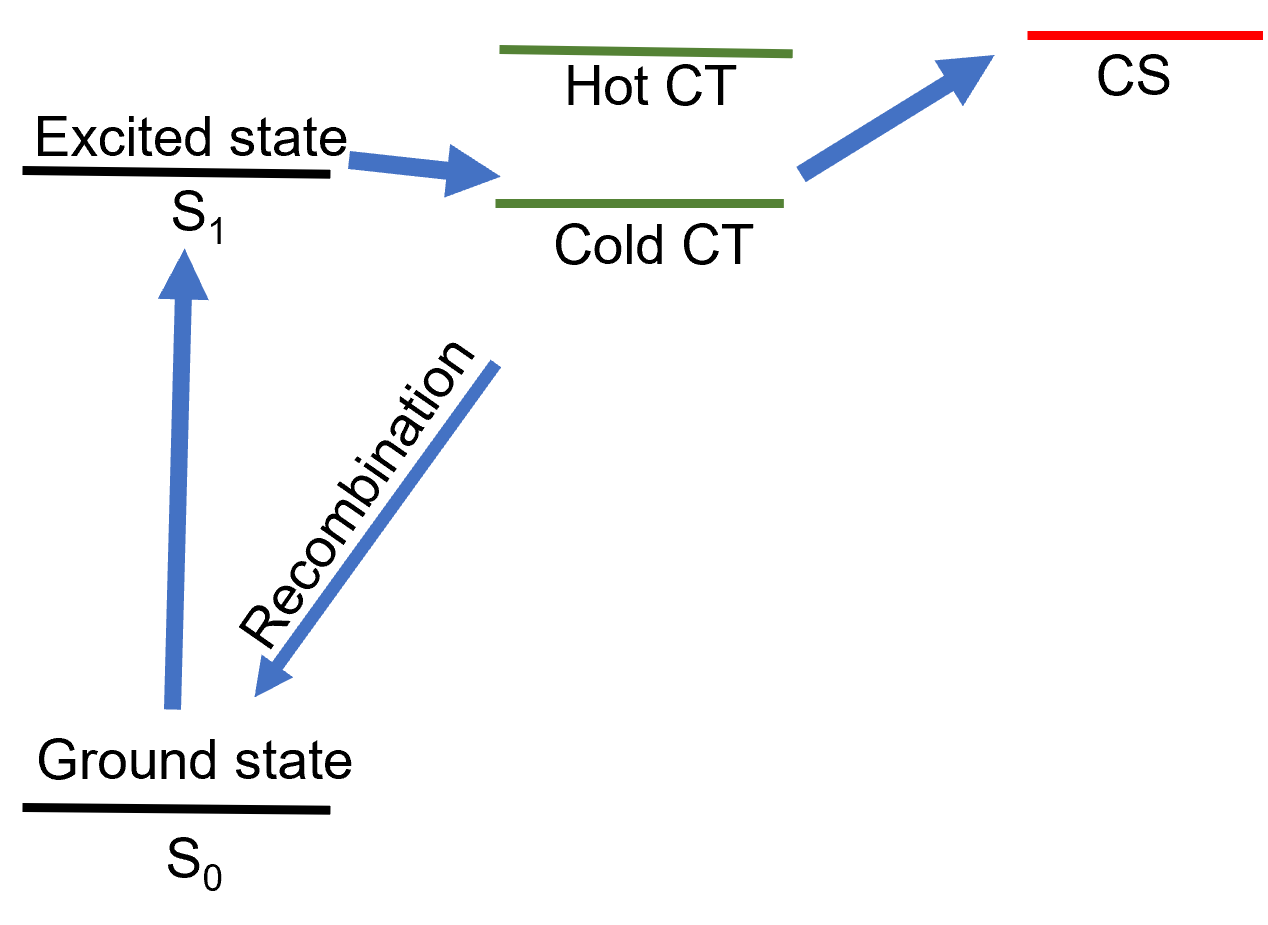
\includegraphics[scale = 0.7]{NFA_hotCT.png}}
\caption{(a) OPV efficiencies in the last two decades. Graph taken from the NREL website \cite{NREL}. (b) Energy uphill CS process in champion OSCs.}
\label{fig:hot and cold}
\end{figure}

However, recently, an exciting breakthrough occurred in the form of NFAs that increased the efficiency of OPVs from 12\% to 18\% in just 3 years (Figure \ref{fig:NREL}). In such OPVs, even though the energy level offset at the D-A interface is small, free charges are generated with a high yield \cite{cheng2018next,hou2018organic,chen2018efficient}. This results in the gain of high photocurrent and large $V_{oc}$ simultaneously, which leads to higher efficiency in such devices. For the OPVs based on these NFAs, efficiency as high as 20\% is predicted \cite{li2018analyzing}.  The NFAs have some advantages over the fullerene acceptors, such as having band gaps in the near-IR region, but how it manages to overcome the fundamental limit in efficiency set forth by the strong exciton binding found in organic materials and what is the uniqueness of these NFAs compared to the traditional fullerene acceptors is still not clear. 
\vspace{7pt}

The CS mechanism in these NFA OPVs cannot be explained through the dissociation of hot CT excitons since the energy offset in these interfaces is relatively lower, which can not offer sufficient energy to the initial S$_1$ excitons to access the hot states. In these recently discovered NFA-polymer BHJs, the S$_1$ excitons are almost in resonance with the cold CT excitons. Therefore, CS can occur only through the dissociation of cold CT excitons, which is an energy uphill and slow process considering their binding energy in the range of around 0.1 to 0.5 eV (see Figure \ref{fig:NFAhot CT}). However, the observed CS time in these NFA BHJs is slower than the CS time of the hot CT excitons (< 1 ps) but 10 - 100 times faster (10ps - 100 ps) than the CS time of the cold CT excitons observed in traditional fullerene BHJs.  \cite{qian2018design,dimitrov2019spectroscopic,menke2018order,liu2018unexpectedly}. In this proposed work, we aim to understand why NFAs can exhibit these attractive features that have not been found in fullerene acceptors by studying the different D-A interfaces and get an insight on improving the photo-to-electrical conversion. 

\section{Hypothesis}
To understand the CS process in NFA BHJs, it is necessary to first identify the driving force responsible for the enthalpy uphill CS. Mathematically,
\begin{equation}
    \Delta F = \Delta E - T\Delta S
\end{equation}
where, ($\Delta F$) represents the change in Gibbs free energy in a system due to change in enthalpy ($\Delta E$) and entropy ($\Delta S$) at a particular temperature ($T$). An enthalpy uphill process can occur much more rapidly if the increase in the enthalpy is compensated by the decrease in the free energy, originating from the entropy gain. In the literature, this is referred to as the entropic driving force \cite{clarke2010charge,monahan2015direct,gregg2011entropy,hood2016entropy}. The previous models on the entropic driving force cannot explain why such force is manifested more effectively at the NFA interfaces than the fullerene interfaces. We argue that the inability of the previous entropy models to explain the CS process in NFAs originates from two fundamental shortfalls;
\begin{itemize}
    \item Most models treat an electron as a localized particle that resides on a single molecule
    \item These models do not incorporate the role of structural anisotropy which are commonly found in organic crystals and polymers
\end{itemize}


Electronic wavefunctions are produced in molecular assemblies as a result of intermolecular coupling \cite{bredas2004charge,scholes2006erratum}. For example, manifold of CT states having a range of binding energies ($\sim$ 0.1 eV - 0.5 eV) and electron delocalization sizes ($\sim$ 1 nm - 4 nm), due to intermolecular coupling, has been observed in previous research work conducted in our lab \cite{wang2017multidimensional}. The delocalization of electrons along with the geometric constraint due to the anisotropy in the electronic coupling can lead to a significant increase in the number of available CT states as a function of energy (density of states, DOS) which increases the entropy function ($S(E)$). Recent study done in our lab has shown that the entropic driving force becomes stronger when the delocalized electron and hole wavefunctions in the CT exciton have a smaller spatial contact area and an enthalpy uphill ($\sim$ 0.3 eV) CS can occur in just a few picoseconds, which is in similar time scale reported in the literature for NFA BHJs \cite{kafle2020spontaneous}. The energy flow is reversed if the entropic driving force is larger than the enthalpy change, allowing the CT excitons to gain energy from the environment. We refer to this process as the \lq{CT exciton heating}' process. Since the free energy of the system increases as the free electron hole pairs are converted back to the bound excitons, this process of exciton heating should not favor the nonradiative recombination and hence minimize the associated energy loss. Indeed, in NFA OPVs, the nonradiative recombination, which is a major cause for the energy loss, appears to be suppressed \cite{ostroverkhova2016organic}.
\begin{figure}[H]
\centering
\subcaptionbox{\label{fig:NFA scheme}}{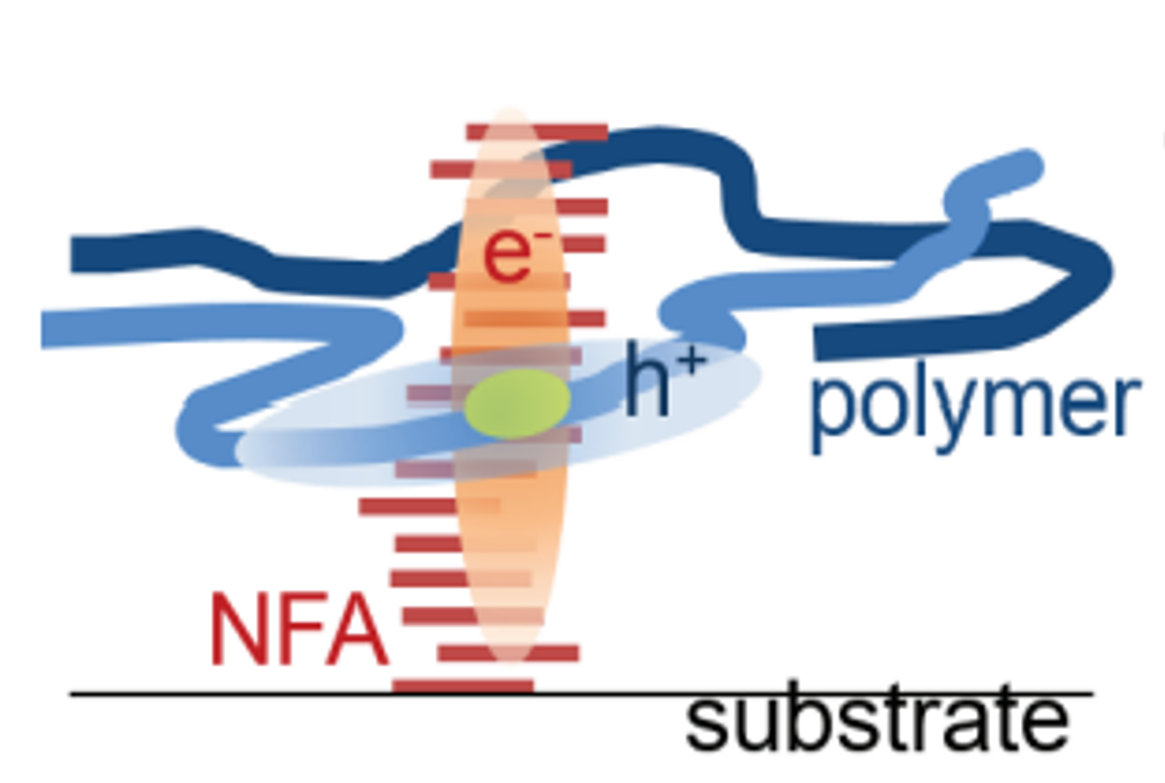
\includegraphics[scale = 0.5]{NFA-scheme.png}} \hspace{60 pt}
\subcaptionbox{\label{fig:FA scheme}}{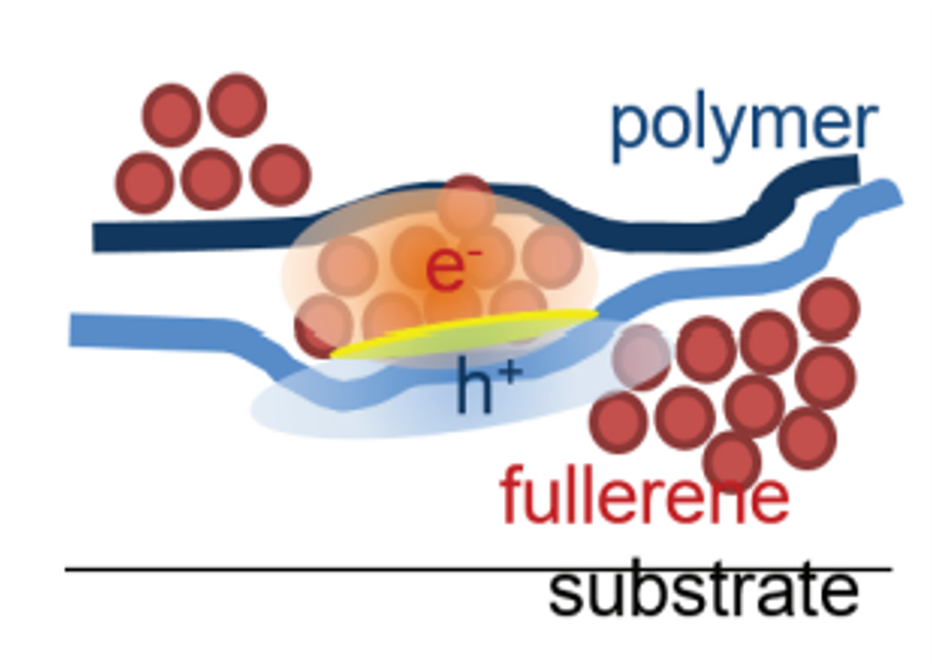
\includegraphics[scale = 0.57]{FA scheme.png}}
\caption{Schematic diagrams showing the structure of (a) 
NFA BHJs and (b) fullerene BHJs. In NFA BHJs, the D-A domains intersect each other at some point-like junctions (yellow spots). The delocalized electron and hole have a more extended contact area in fullerene BHJs.}
\label{fig:NFA and FA}
\end{figure}

There is a major structural difference between polymer/NFA and polymer/fullerene BHJs. In the case of fullerene/polymer BHJs, CS occurs in the D-A intermixed regions where fullerene clusters are intercalated between polymer chains \cite{causa2016fate}. These polymer chains can be expected to wrap around nano-sized, isotropic fullerene domains which significantly increases the contact area between the delocalized electron and hole wavefunctions (see Figure \ref{fig:FA scheme}). In such configuration, entropic driving force is not enough to overcome the enthalpy increase and cooling of hot excitons are expected to occur. On the other hand, in recent years, numerous reports on the structural characterizations of champion polymer/Y6 BHJs have revealed that planar Y6 molecules stack on top of each other along the normal direction and there is a small spacing ($\sim$ \SI{3.5}{\angstrom}) between them \cite{liu202018,zhang2020delocalization,zhu2020crystallography}. Such orientation and spacing can result in a strong nearest neighbor electronic coupling and electron delocalization. On the other hand, the polymer chains where hole wavefunctions delocalize, lie parallel to the substrate. NFA and polymers form nano-fibrous domains that are tangled with each other as shown in Figure \ref{fig:NFA scheme} which makes the delocalized electron and hole wavefunctions look like two 1D strings mostly oriented orthogonal to each other. Such orientation limits the spatial contact area of the electron and hole wavefunctions to some isolated \lq{hot spots}' where they intersect \cite{zhang2020delocalization}. As a result, the minimal contact between the delocalized electron and hole should result in a DOS function that favors the CT exciton heating process.
\vspace{7pt}

To summarize, we argue that the crystal packing at the nano-scale determines whether the energy uphill CS mechanism can occur or not. Certain nanostructures like the ones found in the champion polymer/Y6 OPVs can offer a larger DOS function, which should favor the CT exciton heating process. To test these hypotheses, we want to create different interfaces having different nanopatterns and study the CS using ultrafast spectroscopy techniques to understand the CS mechanism.

\section{Experimental methods}
In our lab we employ different experimental techniques to characterize samples and study their electronic properties using different spectroscopy techniques such as photoemission spectroscopy (PES) and absorption spectroscopy. A brief description of some of the experimental techniques which we have used in the past and which we will be extensively using for our future works is explained in the following subsections. 

\subsection{Low energy electron diffraction (LEED) experiment}
LEED is a relatively inexpensive and fast technique for determining the surface structures and geometries of materials and is based on the wavelike properties of electrons. Ever since its discovery the phenomenon of electron diffraction has evolved into a powerful technique for the determination of surface structures. In particular, the low-electrons having energies less than several hundred electron volts have elastic mean free paths measured in angstroms (\SI{}{\angstrom}), making it particularly sensitive to surfaces. For this reason, LEED is widely used and is one of the most common techniques for determining surface structures and geometries \cite{watson2003nist,van2009atomic,soares2011advances}. A schematic diagram of LEED imaging is shown in Figure \ref{fig:3a}. It consists of an electron gun which directs a collimated mono-energetic beam of electrons towards the surface of the sample. The diffraction pattern of the elastically back-scattered electrons is produced in the luminescent screen and the image of the screen is taken with the help of a CCD camera.


\begin{figure}[H]
\centering
\subcaptionbox{\label{fig:3a}}{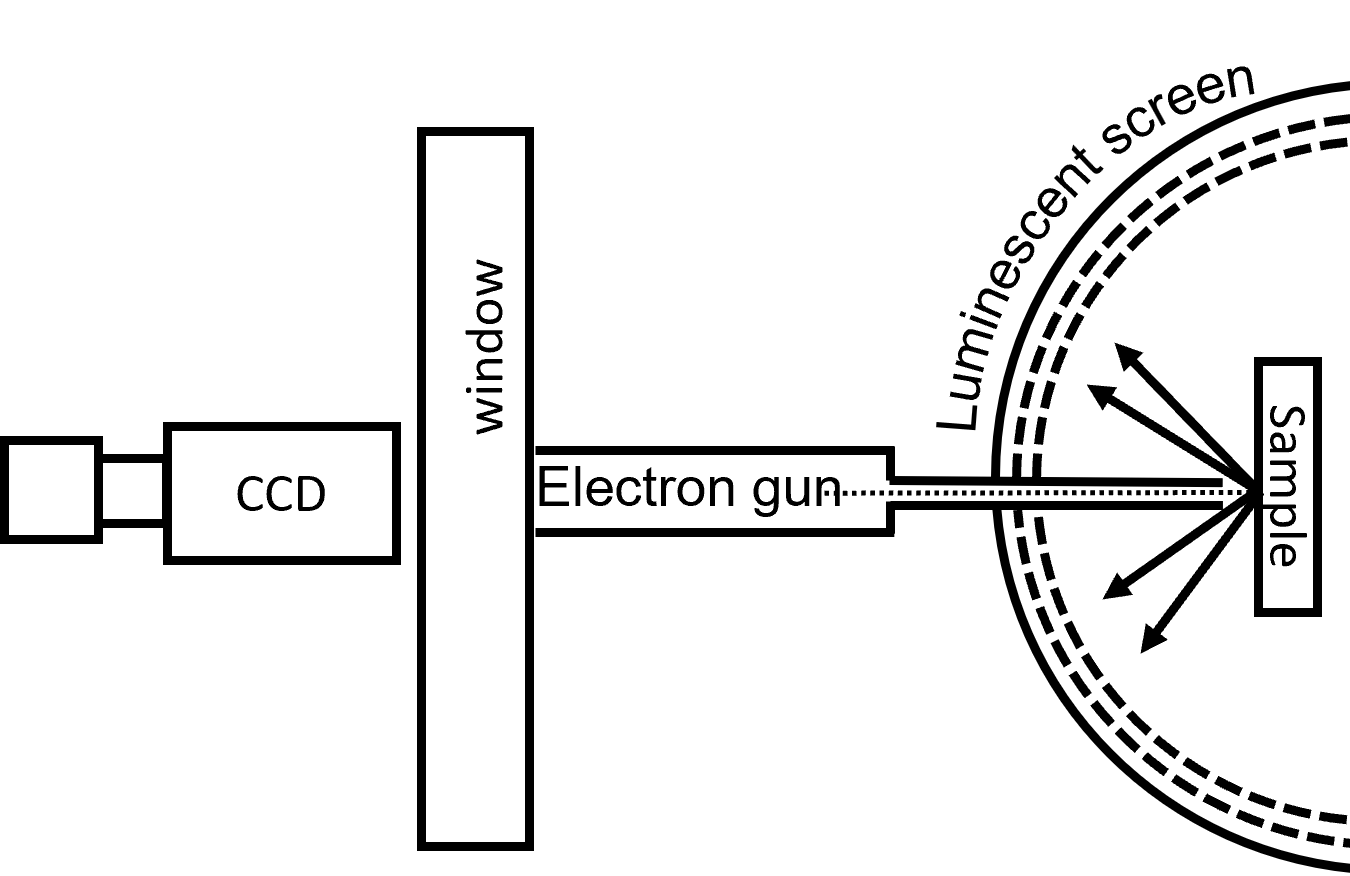
\includegraphics[scale = 0.68]{LEED_schematic_copy.png}}\quad \hspace{45pt}
\subcaptionbox{\label{fig:3b}}{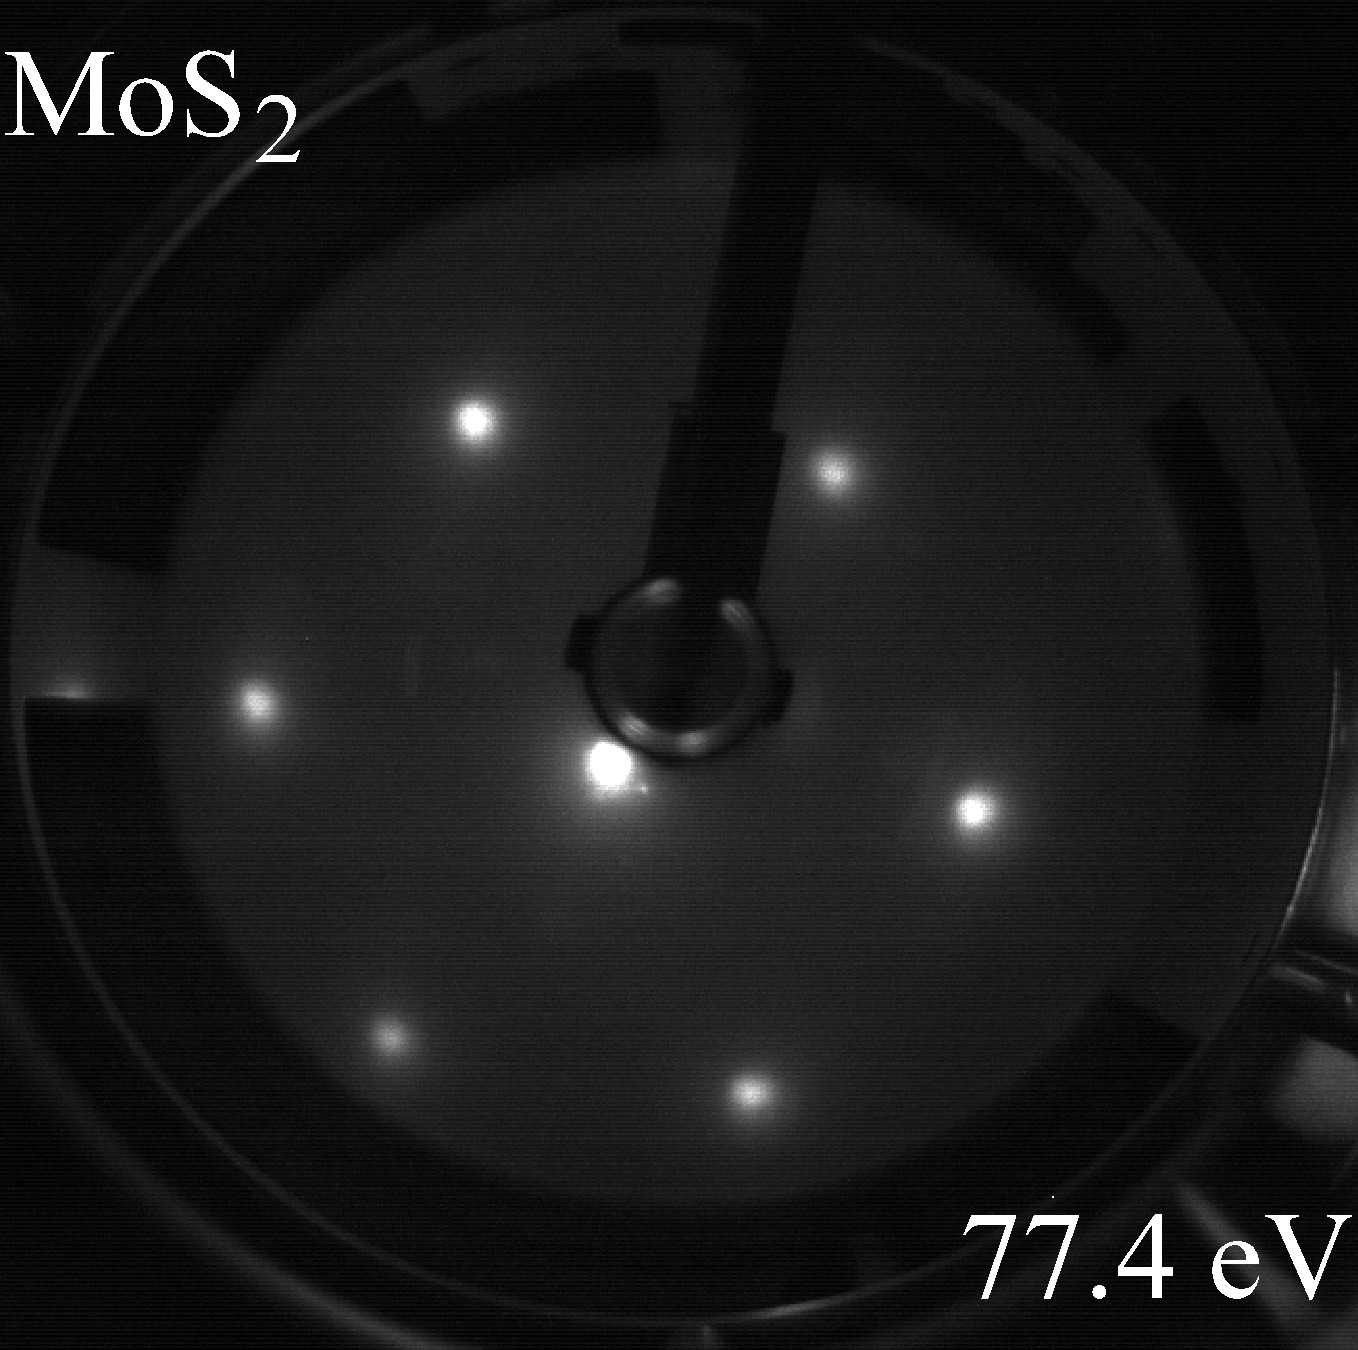
\includegraphics[width=3.55cm]{MoS2_77_4eV.pdf}}
\caption{(a) Schematic diagram of LEED measurement. (b) LEED image of bulk MoS$_2$ at 77.4 eV (K.E. of electrons).}
\end{figure}

Because of the short penetration depth of low-energy electrons, the diffraction process is determined by a small number atomic layers at the crystal surface. Therefore, in LEED the array of relevant scatterers is only periodic in two dimensions. When the wavelengths of the incident low-energy electron waves are comparable to the lattice parameters of the crystals, the phenomenon of interference occurs between the scattered waves and diffraction spots can be seen in the screen (e.g. Figure \ref{fig:3b}). LEED images give the measurement of lattice vectors in reciprocal space which can be converted back to the real space to obtain the lattice parameters ($a_1$, $a_2$) and the angle ($\theta$) between the lattice vectors. This technique also makes it possible to measure the relative orientation of one crystal lattice over another when a thin layer of it is placed directly on top of another crystal.

\subsection{UPS Experiment}

UPS is based on photoemission technique and is a standard method for the investigation of electronic states in metals and semiconductors. It probes the valence states near the Fermi level, which plays an important role in molecular bonding and charge transport. For the energy range of UV photons used in UPS, the escape depth of electrons is only around $\sim$ 1 nm – 2 nm which means the UPS technique is able to detect the electrons coming out from the top surface only. For this reason, the UPS measurement must be done inside an ultra-high vacuum chamber (UHV), and the sample must be atomically clean and free from any adsorbed contaminants. Thus, UPS studies can provide information on the surface electronic states of the valence band of the molecules used in our experiments. 


\begin{figure}[H]
\centering
\subcaptionbox{\label{fig:UPS scheme}}{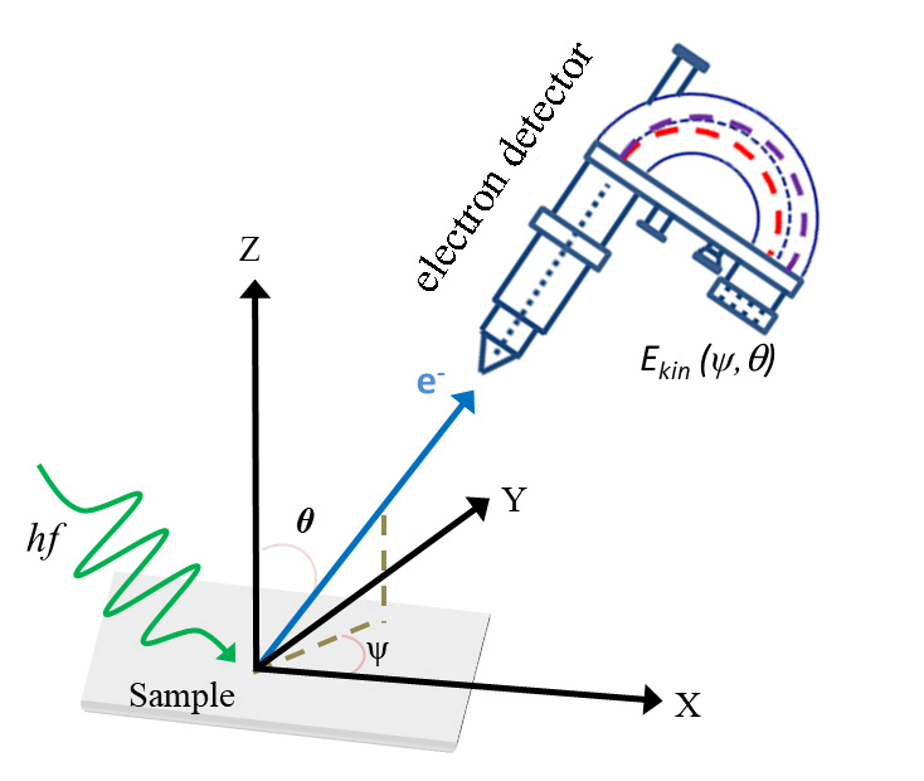
\includegraphics[scale = 0.55]{UPS-Detector.png}}
\subcaptionbox{\label{fig:UPS plot}}{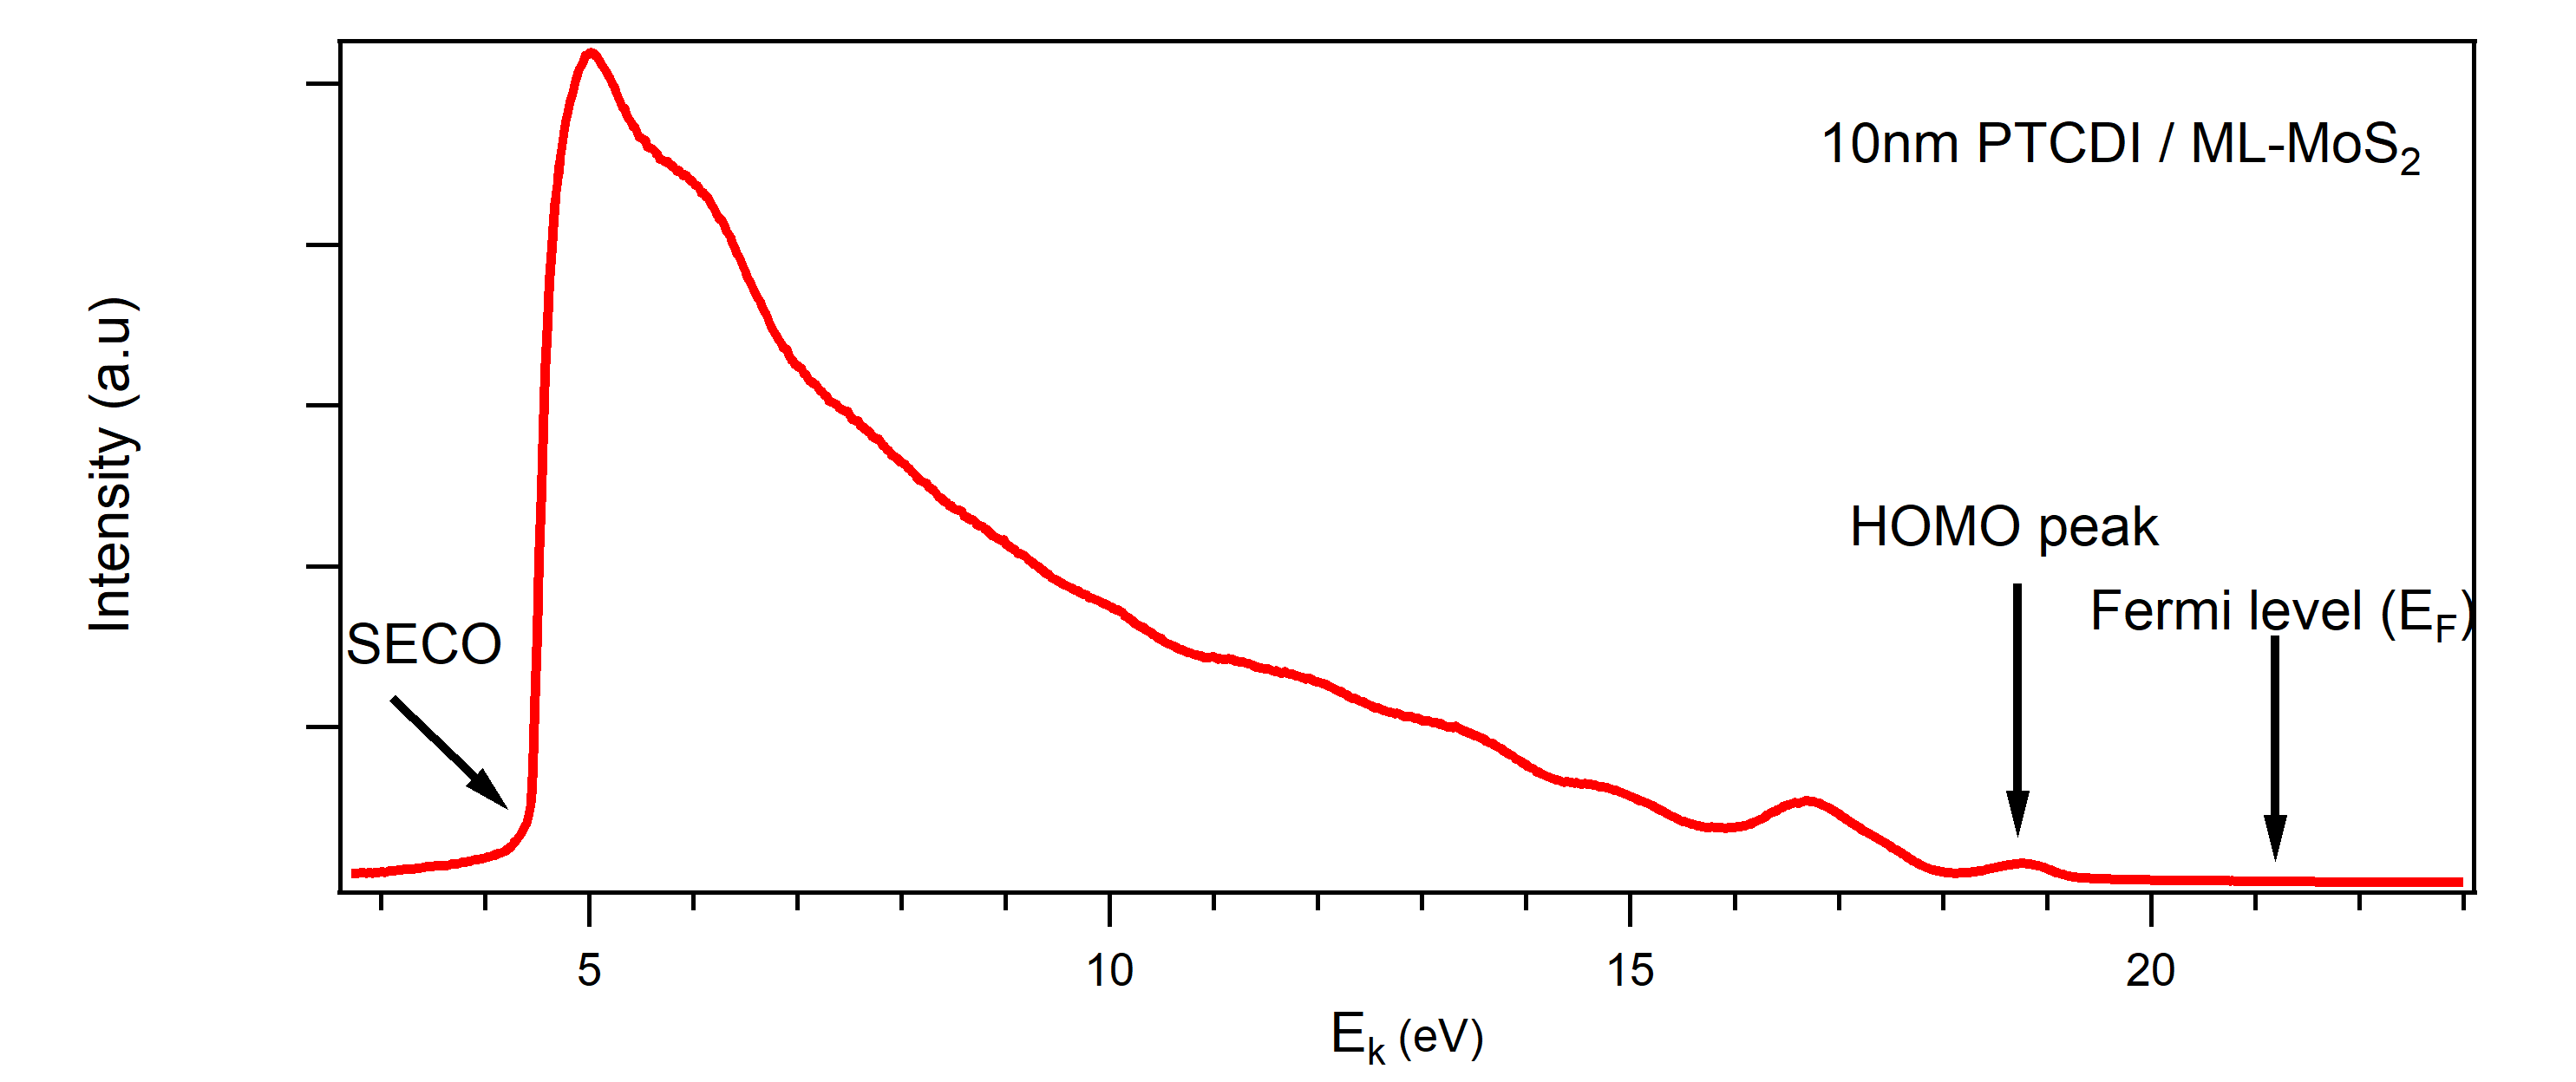
\includegraphics[scale = 0.51]{example_UPS.png}}
\caption{(a) Schematic diagram of the UPS technique. (b) UPS spectra of 10nm PTCDI/ML-MoS$_2$ showing secondary electron cut-off (SECO), HOMO peak and fermi-level.}
\label{fig:UPS method}
\end{figure}


This technique uses a UV lamp to generate the UV photons that eject the electrons from the valence band of a material to the vacuum levels. The measurement of intensity and kinetic energy ($E_k$) of the photo-emitted electrons is done with the help of a hemispherical electron analyzer (see Figure \ref{fig:UPS scheme}). Thus, we can get the graph of photoemission intensity vs. kinetic energy ($E_k$) from the UPS measurement (see Figure \ref{fig:UPS plot}). This plot enables us to determine the binding energy ($E_B$) and the possible electronic states from which they are ejected before photoemission. The $E_B$ can be determined with the help of the following energy conservation relation:

\begin{equation}
    E_k = hf - E_B
    \label{eqn:energy_conservation}
\end{equation}

\noindent where $f$ is the frequency of the UV light.
\vspace{7pt}

UPS studies are also commonly used to find the work function ($\Phi$) and ionization potential ($IP$) of the sample. In solid-state physics, $\Phi$ is defined as the minimum amount of energy needed to remove an electron from a solid to a point in the vacuum immediately outside the solid surface, while IP is the energy required to remove the outermost electron in an atom in its ground state to infinity, i.e. cause the atom to become ionized. They can be calculated using the following equations.

\begin{equation}
    \Phi = hf - |E_k - E_f|
    \label{eqn:phi}
\end{equation}
\begin{equation}
    IP = hf - |SECO - HOMO_{peak}|
    \label{eqn:IP}
\end{equation}

Here $hf$ corresponds to the energy of the UV source (He-I transition).

\subsection{TR-TPPE experiment}
\begin{figure}[H]
    \centering
    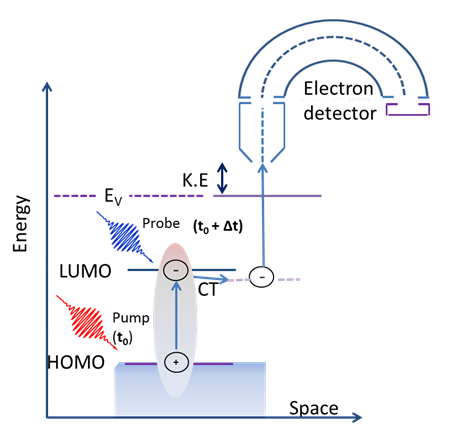
\includegraphics[width = 9cm]{TPPE scheme TIKA.png}
    \caption{Schematic diagram of TPPE measurement \cite{kafle2019role}.}
    \label{fig:TPPE scheme}
\end{figure}
TR-TPPE is another photoemission-based technique, which allows us to study the unoccupied states in metals and semiconductors. This method utilizes two femtosecond laser pulses, which are referred to as the pump pulse and the probe pulse. The pump pulse excites the electrons from their ground state (HOMO) to the unoccupied intermediate excited state (LUMO), and the probe pulse kicks out the excited-level electrons to the vacuum level ($E_v$) after a certain delay time. And finally, the Kinetic energy ($E_k$) and the intensity of the emitted photo-electrons are measured with the help of a CCD camera, equipped in the hemispherical electron analyzer. We can determine the binding energy ($E_B$) of the intermediate excited states by using the energy conservation relation in equation \ref{eqn:energy_conservation}. The schematic diagram of the TR-TPPE experiment is shown in Figure \ref{fig:TPPE scheme}.



\begin{figure}[H]
\centering
\subcaptionbox{\label{fig:2Dspectra}}{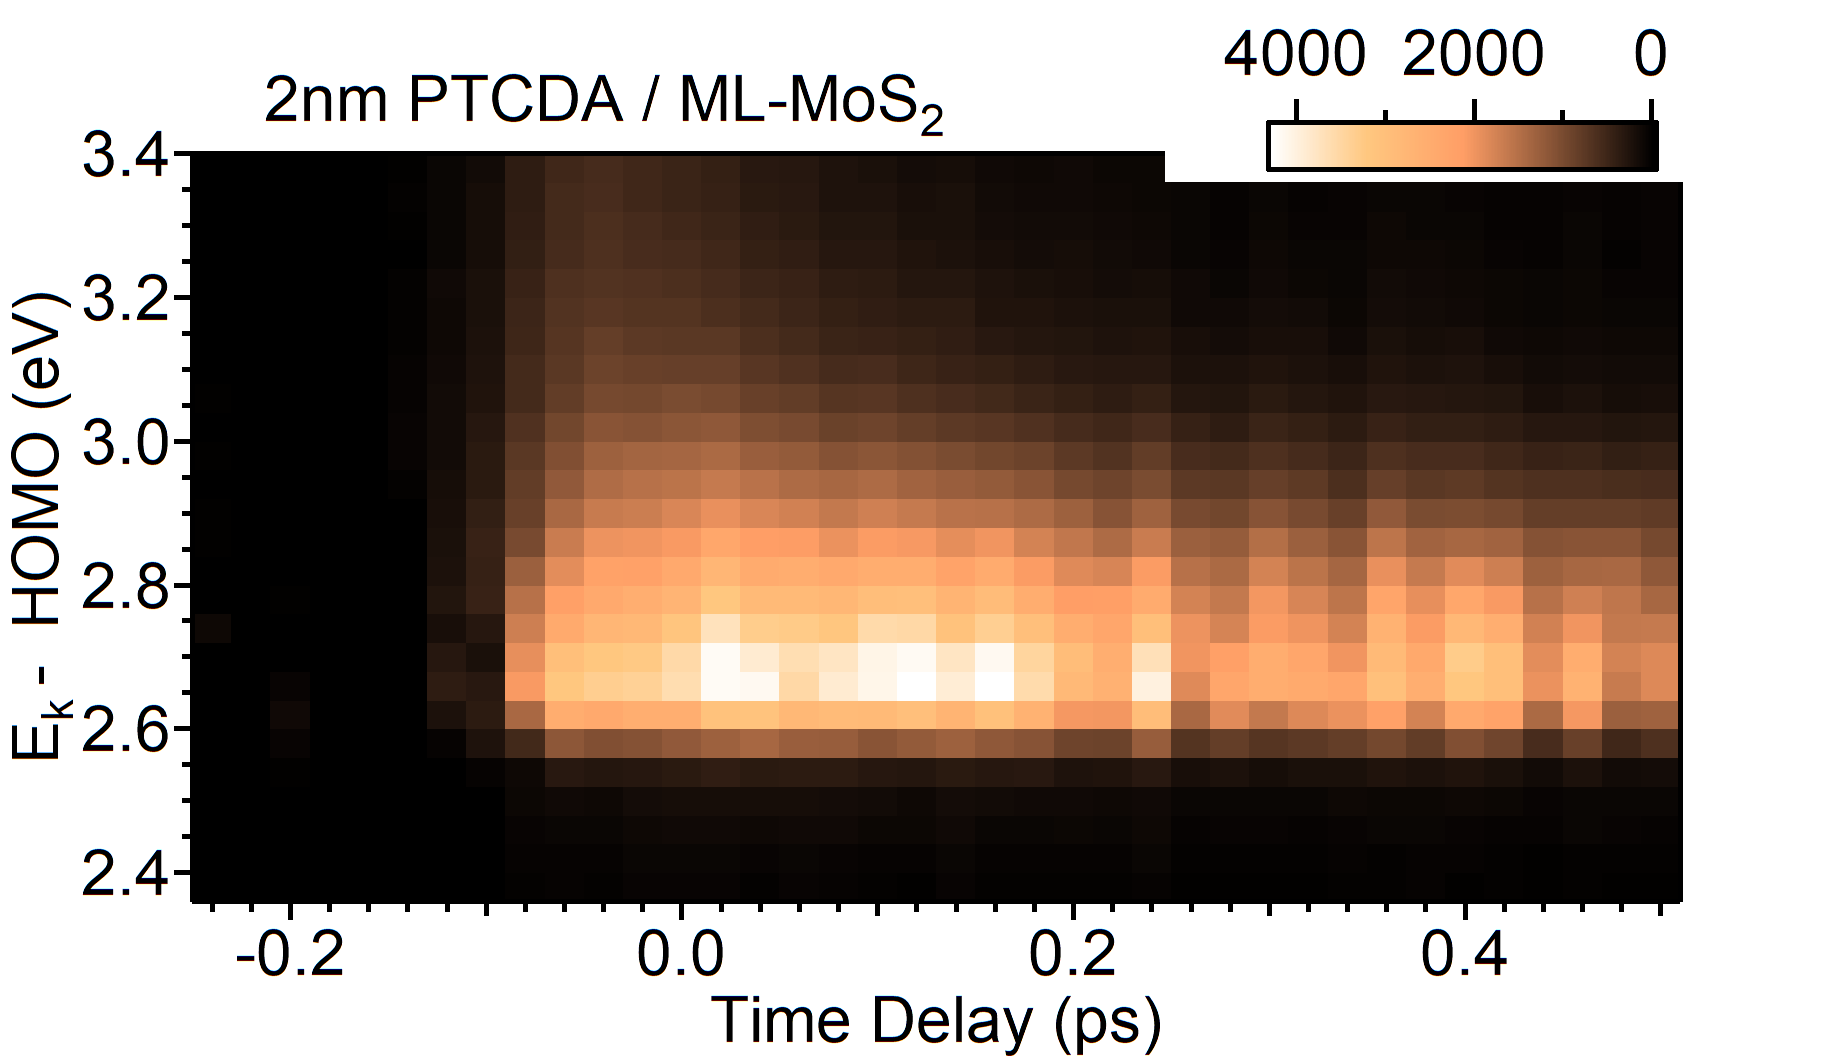
\includegraphics[width=10cm]{TPPE example 2D.png}}\vspace{0.5cm}
\subcaptionbox{\label{fig:timecut}}{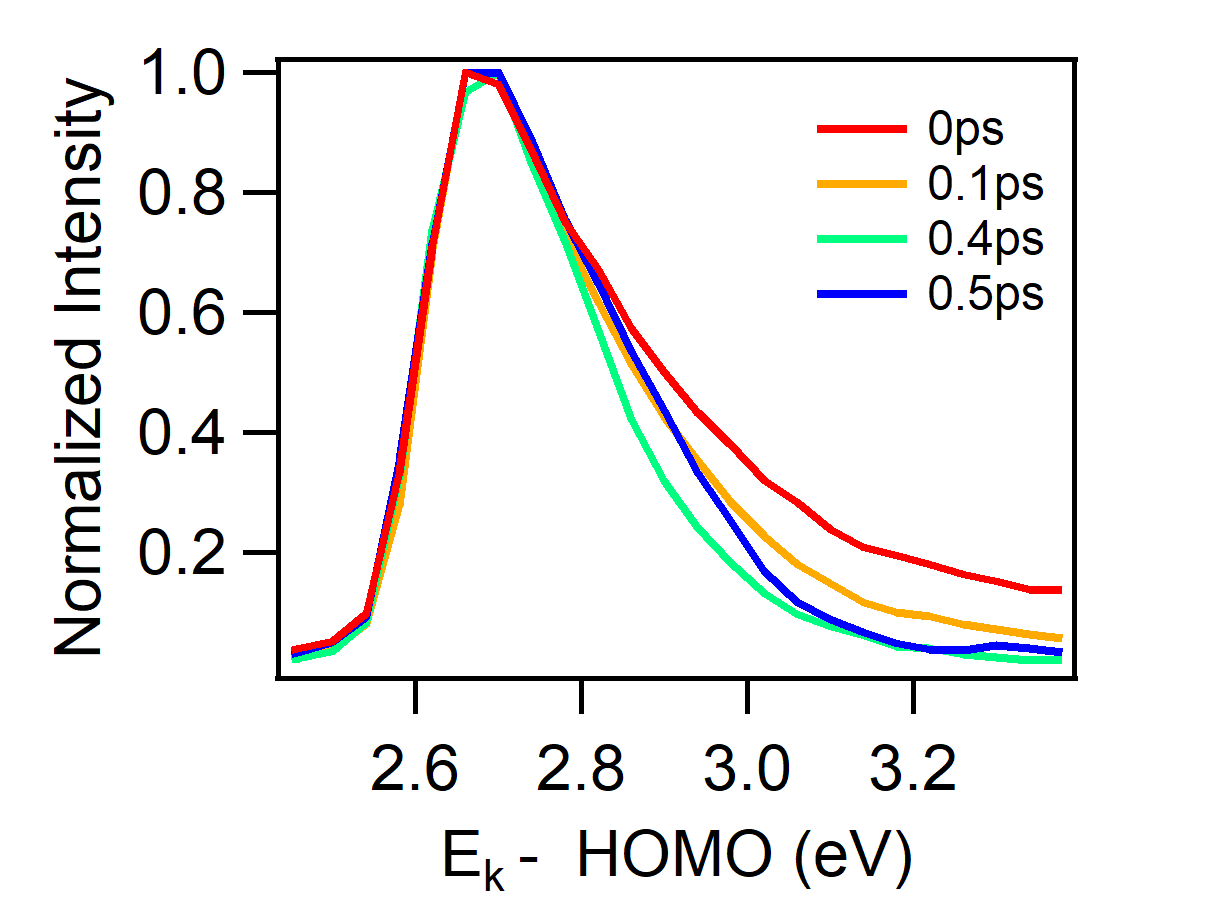
\includegraphics[width=6.5cm]{timecut.png}} \hspace{0.3cm}
\subcaptionbox{\label{fig:energycut}}{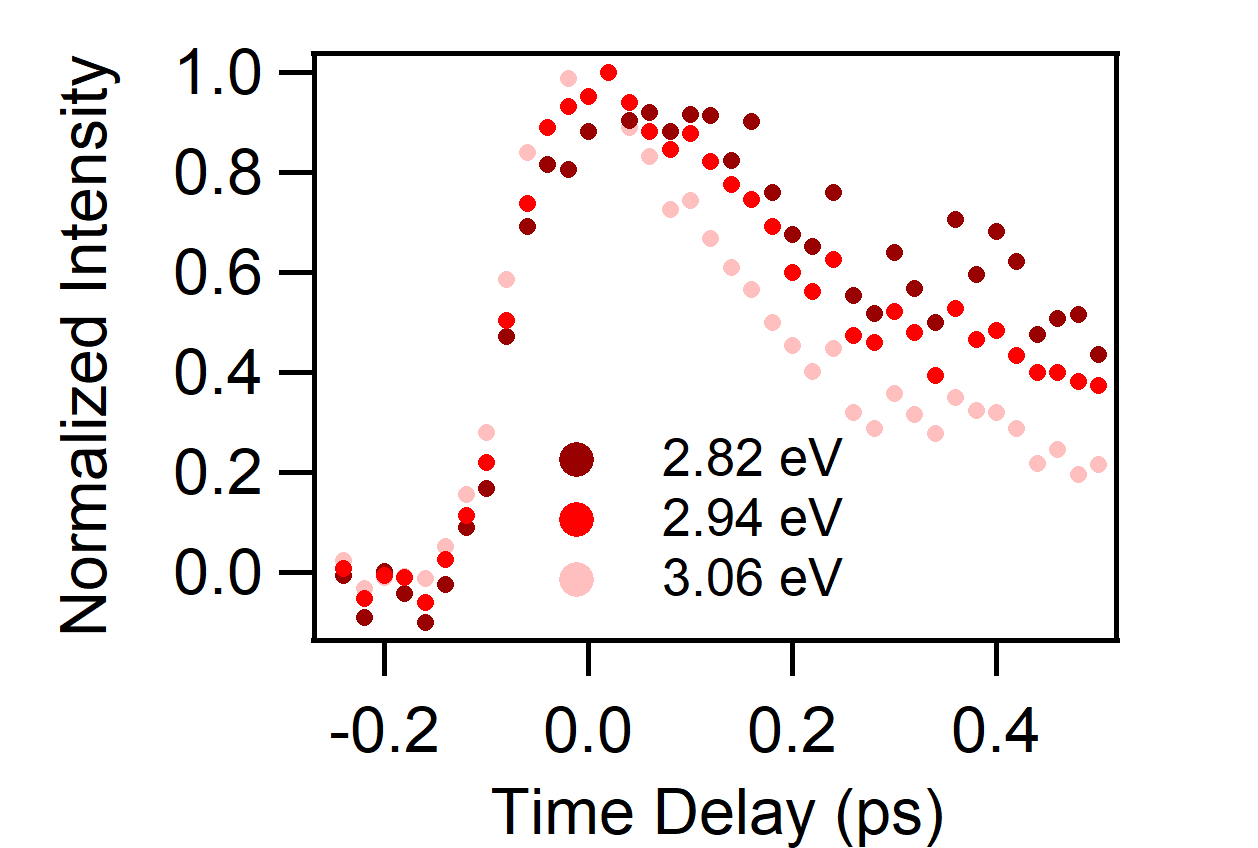
\includegraphics[width=6.5cm]{energycut.png}}

\caption{TR-TPPE spectra from 2nm PTCDA / ML-MoS$_2$ showing (a) 2D plot and (b) its vertical cut and (c) horizontal cut.}\label{fig:TPPE 2D}
\end{figure}

By introducing a continuously varying time delay between the two pulses in the experiment, we can measure the lifetime of the excited states with the resolution in the order of tens of femtoseconds. A typical 2D plot obtained from the TR-TPPE measurement is shown in Figure \ref{fig:TPPE 2D}. The horizontal cut of the 2D plot gives the temporal evolution of the population of electrons at a particular energy level in the excited state while the vertical cut gives the population of the electrons in different energy levels at a particular time.  Thus, this technique enables us to study the dynamics of the CT process, excitonic decay, and charge separation as well.

\section{Study on the role of nanopatterns and electron delocalization in the rate of charge transfer}
Quick electron transfer from donor to acceptor molecules across the interface of a heterojunction is necessary for effective photo-to-electrical conversion in any photovoltaic or photosensing device. A slow ET at the interface can allow other competitive recombination processes to occur, which can significantly hinder device performance. Different acceptor molecules form different nanopatterns when they are deposited on substrates using vapor deposition technique. These nanopatterns in turn determine the dimensionality and orientation of the electron wavefunction in acceptor molecules, which along with the interfacial band offset ($E_{off}$) between the lower end of the conduction band (CB) of the donor and upper end of the lowest unoccupied molecular orbital (LUMO) of the accceptor molecules should impact the rate of charge transfer across the interface. In order to study these effects, we conducted controlled experiments on different TMDCs-organic hybrid interfaces. 

\begin{figure}[H]
\centering
\subcaptionbox{\label{fig:hybrid energy level}}{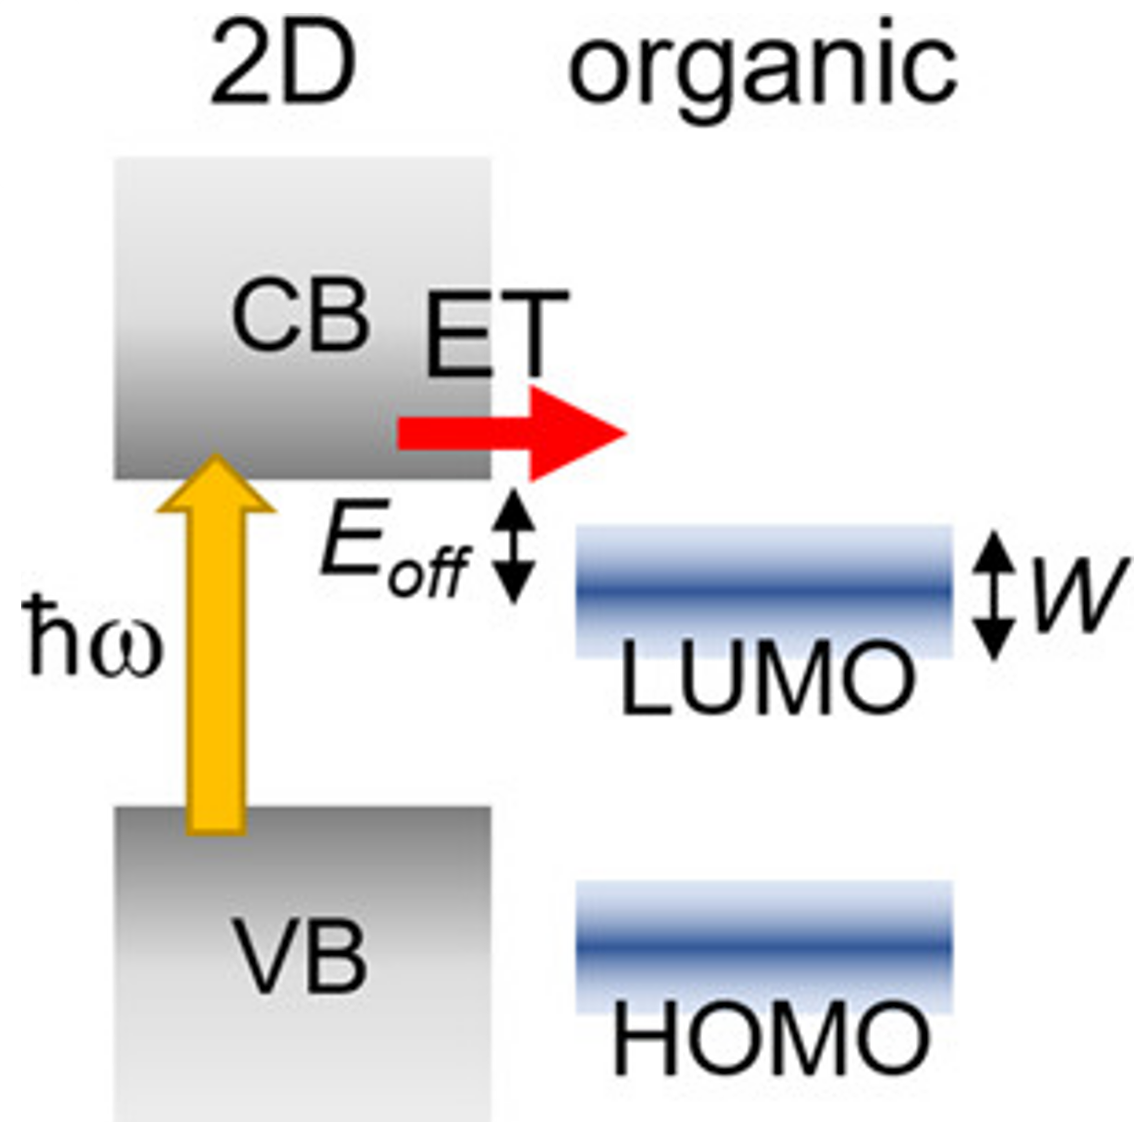
\includegraphics[scale=0.6]{2D-organic.png}} \hspace{20pt}
\subcaptionbox{\label{fig:3D-1D}}{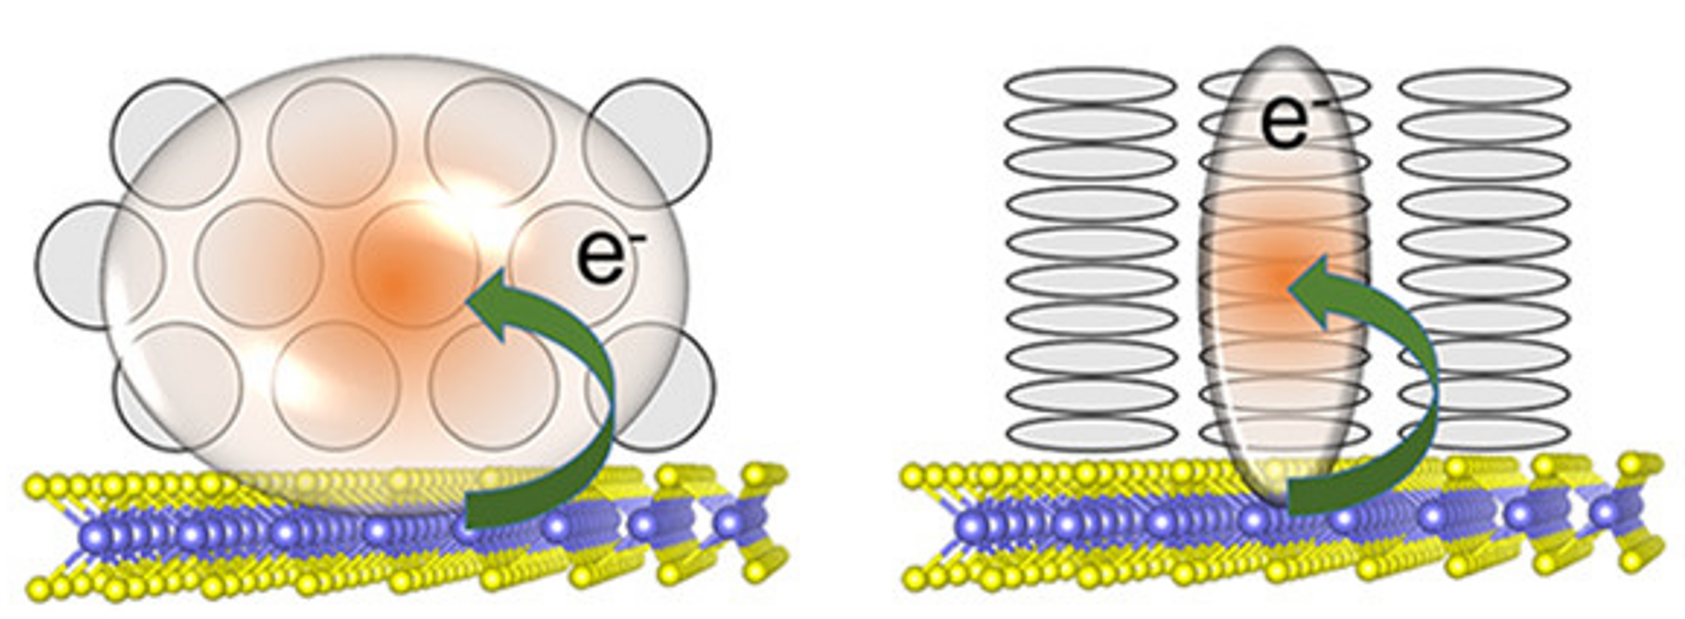
\includegraphics[width=9.5cm]{delocalization_crop.png}} 

\caption{(a) Band alignment and ET at the 2D - Organic hybrid interface. (b) ET from TMDC to Fullerene (left) and NFAs (PTCDA/PTCDI) (right). The electron wavefunction delocalizes in 1D in PTCDA/PTCDI acceptors but in the fullerene acceptors it delocalizes in 3D \cite{rijal2020collective}.}\label{fig:charge transfer scheme}
\end{figure}


In particular, we studied the rate of charge transfer from TMDCs (ML-MoS$_2$ and ML-WSe$_2$) to fullerenes and perylene derivatives (PTCDA and PTCDI). ML-MoS$_2$ and ML-WSe$_2$ have different electron affinity ($\sim$ 0.5eV) which allows us to tune the $E_{off}$ between the molecules at the interface. Fullerenes (C$_{60}$) molecules are known to form face-centered cubic (fcc) crystal structures, while planar PTCDA/PTCDI molecules stack together in 1D columns normal to the surface of the substrate \cite{ching1991first,ludwig1994stm}. According to the tight-binding models that include the nearest-neighbor interaction, fullerenes having a cubic fcc crystal structure and 12 nearest neighbors can have a bandwidth ($W$) which is 6 times larger than that of a 1D array of planar molecules having 2 nearest-neighbor interaction. The presence of two different nanopatterns in these organic acceptors also leads to the two different dimensionality of the delocalized wavefunctions. In the case of planar PTCDA/PTCDI acceptors, the electron wave functions are delocalized in the 1D plane, while in the case of fullerene acceptors, they are delocalized in 3D as shown in Figure \ref{fig:3D-1D}.

\begin{figure}[H]
\centering
\subcaptionbox{\label{fig:UPS_ETrate}}{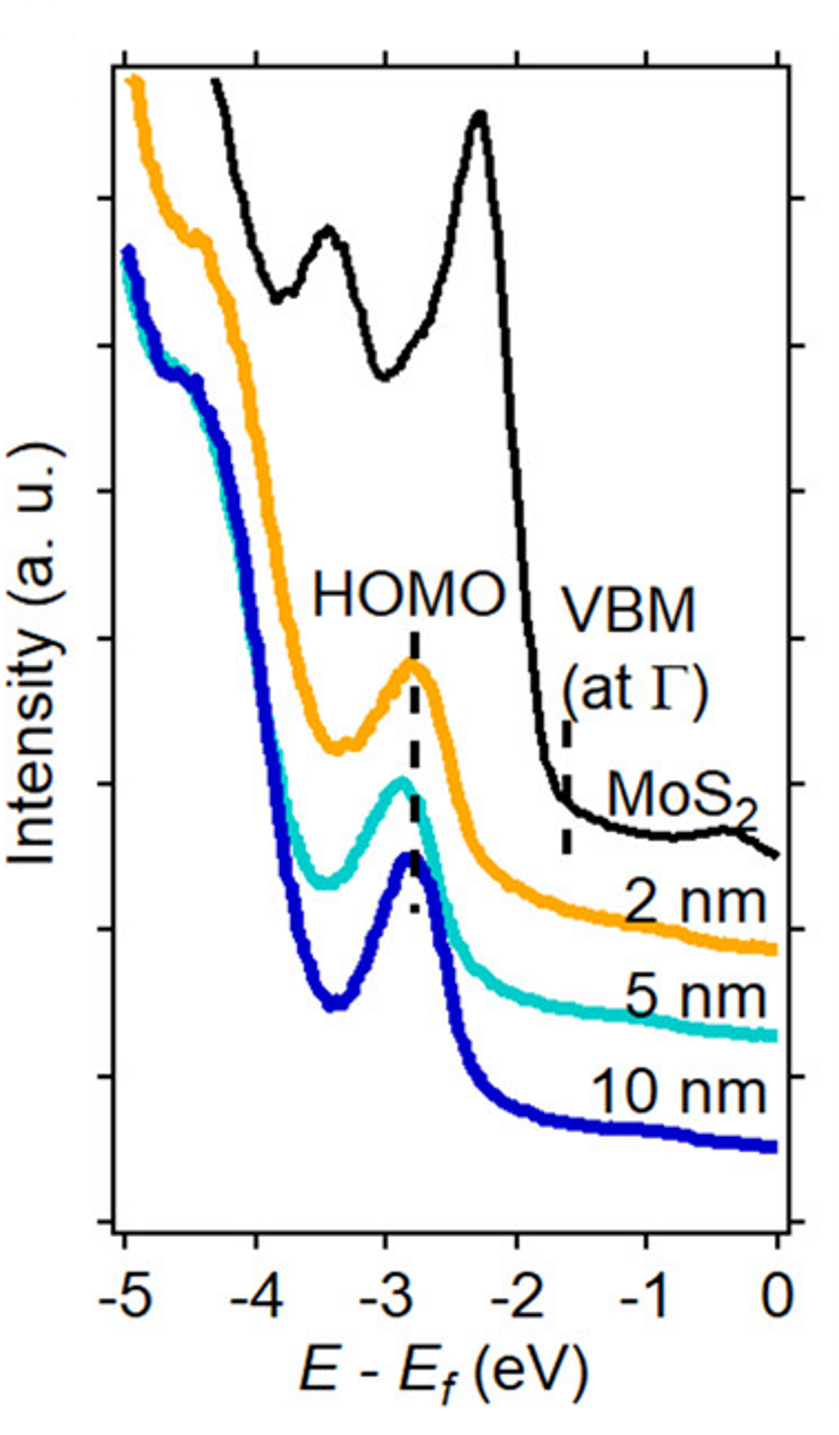
\includegraphics[scale=0.75]{UPS_ETrate.png}}
\subcaptionbox{\label{fig:ET-alignment}}{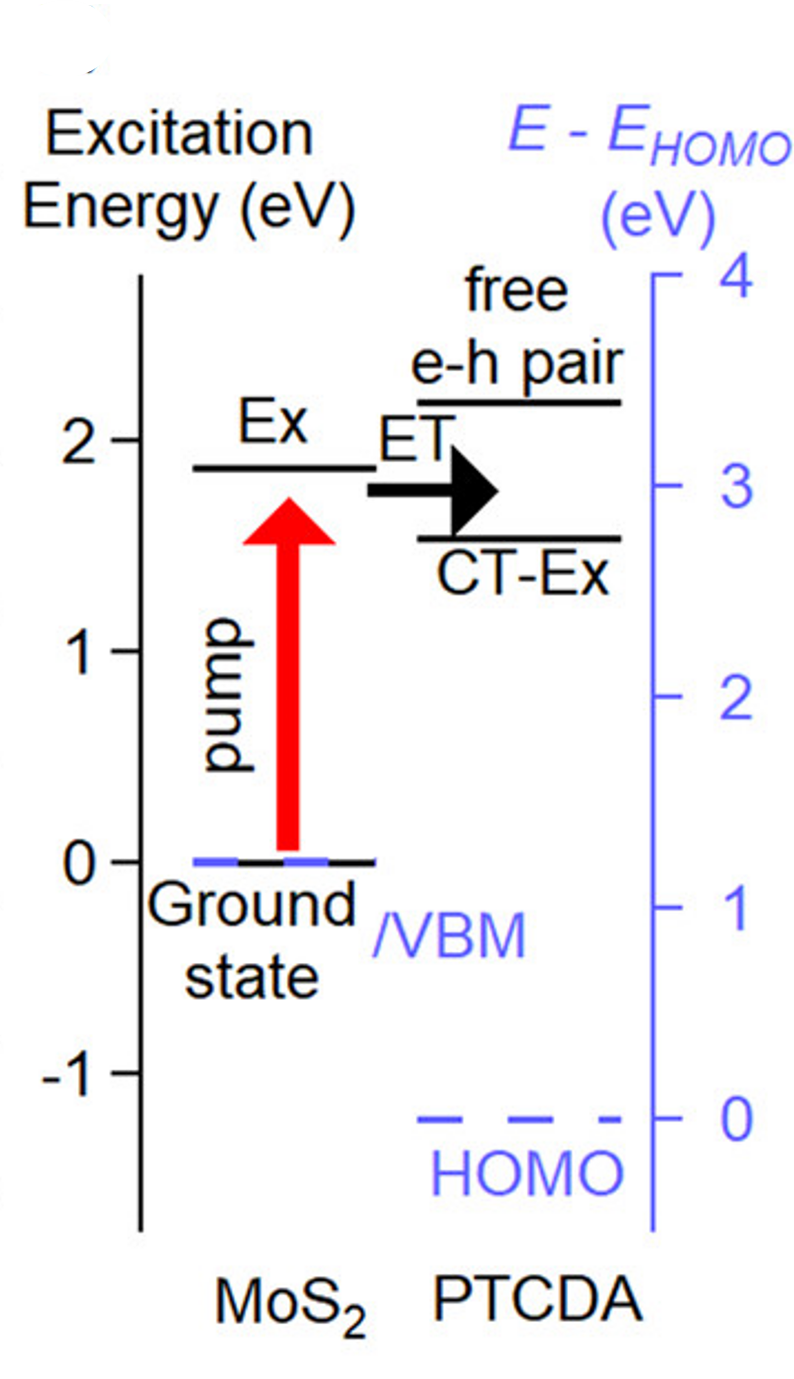
\includegraphics[scale=0.75]{ET-alignment.png}} 
\subcaptionbox{\label{fig:TPPE rate PTCDA}}{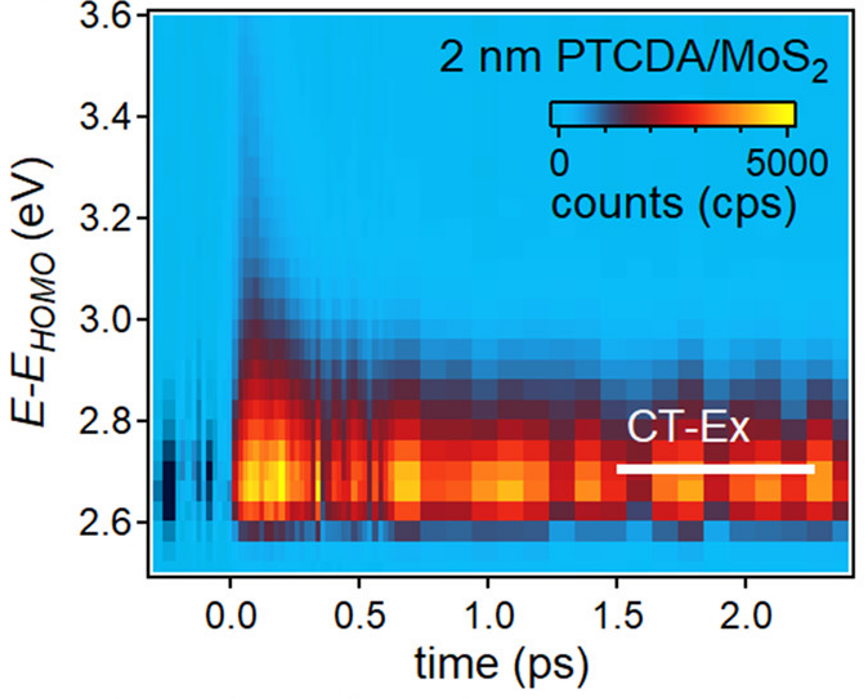
\includegraphics{TPPE rate PTCDA.png}} 
\caption{(a) UPS spectra, (b) band alignment and (c) TR-TPPE spectra of the ML-MoS$_2$ / PTCDA sample \cite{rijal2020collective}.}\label{fig:ET UPS TPPE}
\end{figure}

Different thicknesses of organic molecules were grown on the 2D TMDC substrates inside the UHV chamber with base pressure $\sim 1 \times 10^{-9}$ Torr using the vapor deposition technique. We conducted the UPS and TR-TPPE measurements in the above mentioned interfaces. The UPS spectra and the energy level diagram of ML-MoS$_2$/ PTCDA  is shown in Figure \ref{fig:UPS_ETrate} and \ref{fig:ET-alignment}, respectively. The energy level diagram was plotted using the measured HOMO-VBM offset from UPS spectra and reported values of the optical and transport band gaps of the two materials \cite{martinez2014imaging,forker2009optical,park2018direct}. In the TR-TPPE experiment, TMDCs were selectively photoexcited with the help of a pump pulse of 1.88 eV (for interfaces with MoS$_2$) and 1.77 eV (for interfaces with WSe$_2$) to generate excitons. After the ET from TMDCs to organic molecules, CT excitons are produced in the interface which populates the CT-Ex states via hot CT states. Finally, the electrons in these CT-excitons are kicked out by the UV probe pulse (4.65 eV) after a certain delay stage. A 2D plot of the TR-TPPE spectra from the ML-MoS$_2$ / 2nm PTCDA is shown in Figure \ref{fig:TPPE rate PTCDA}. Finally, the ET rate and the population of these CT excitons at different energy levels and different delay times were studied using the TR-TPPE spectra. In TR-TPPE spectra, the rise time in the signal directly corresponds to the ET time across the interface, which can be determined by fitting a rate equation model with the temporal evolution of the intensity.

\begin{figure}[H]
\centering
\subcaptionbox{\label{fig:PTCDA-MoS2}}{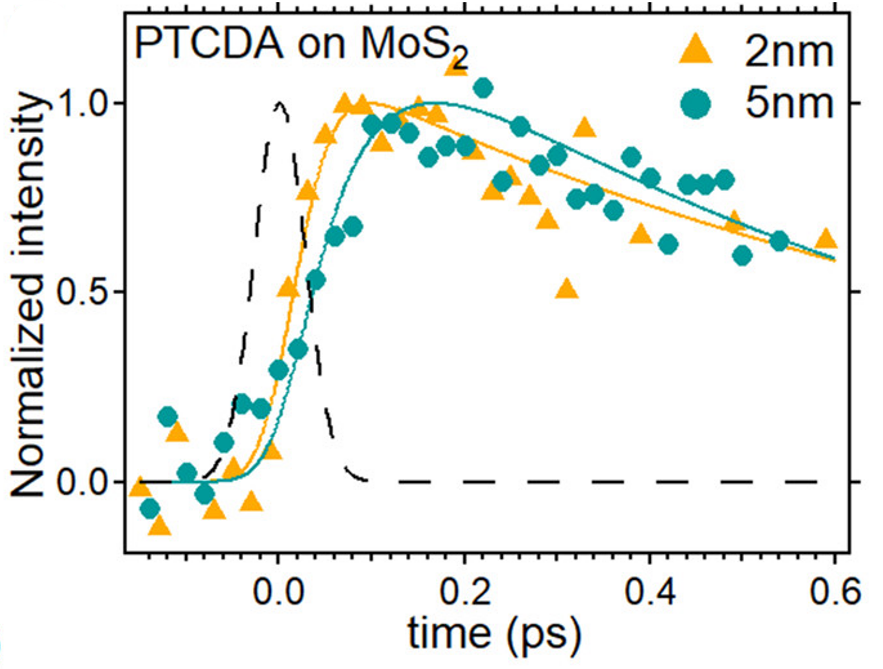
\includegraphics[scale=0.81]{PTCDA-MoS2.png}}\hspace{70pt}
\subcaptionbox{\label{fig:PTCDI-MoS2.png}}{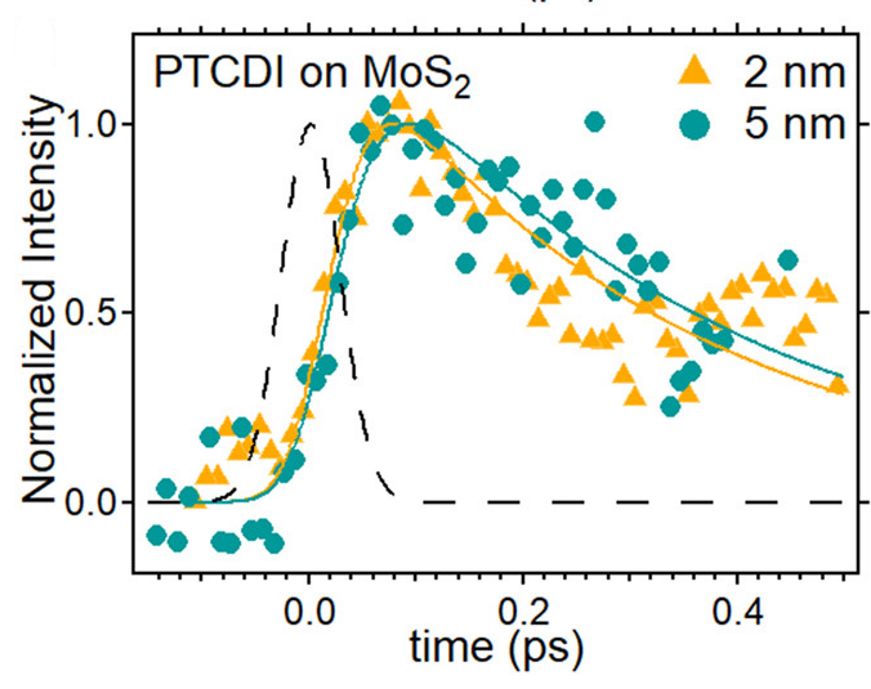
\includegraphics[scale=0.81]{PTCDI-MoS2.png}}
\subcaptionbox{\label{fig:PTCDI-WSe2}}{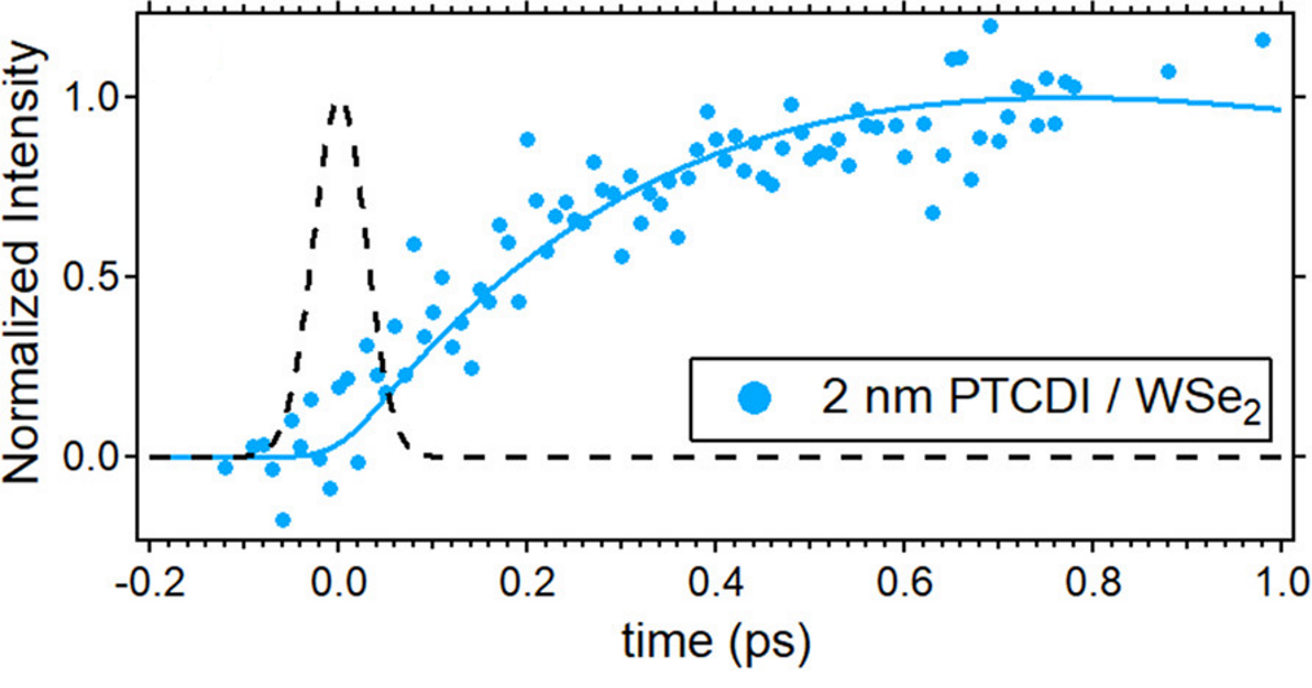
\includegraphics[scale=0.81]{PTCDI-WSe2.png}}
\subcaptionbox{\label{fig:C60-MoS2-WSe2}}{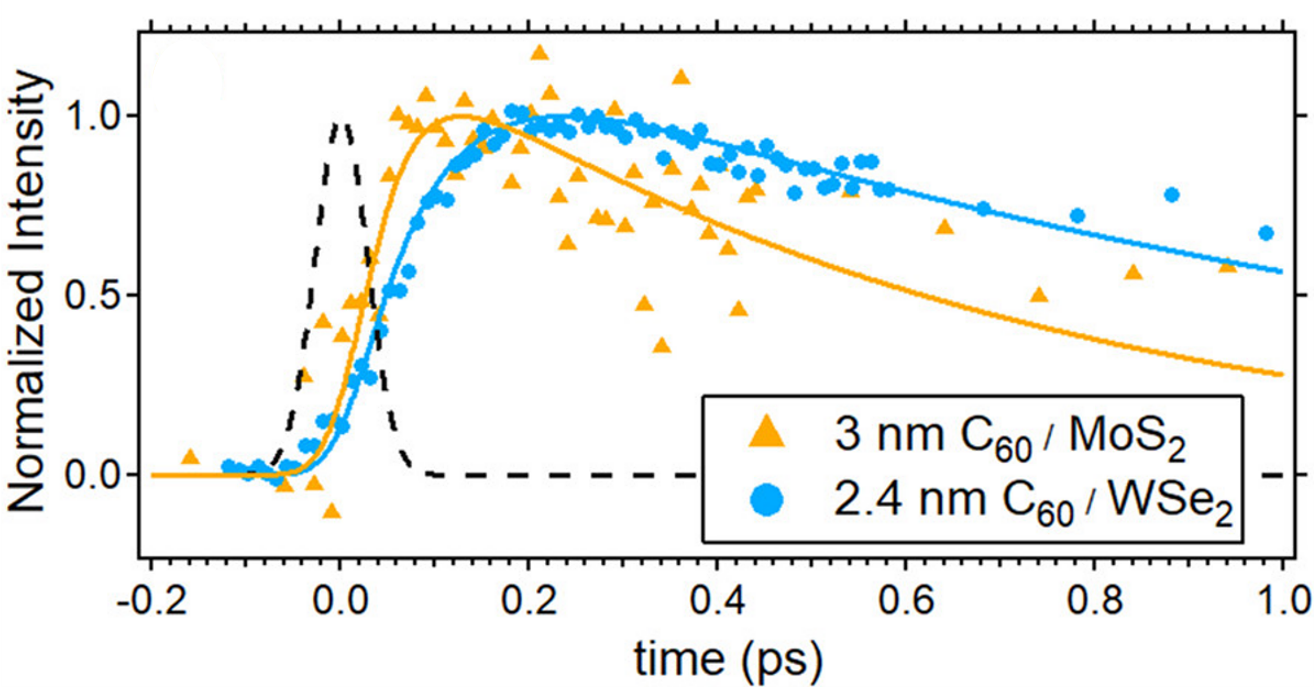
\includegraphics[scale=0.81]{C60-MoS2-WSe2.png}} 
\caption{The fitted ET time for different thicknesses of (a) PTCDA on MoS$_2$, (b) PTCDI on MoS$_2$, (c) PTCDI on WSe$_2$, and (d) C$_{60}$ on MoS$_2$, WSe$_2$. The dotted black lines indicate the pump-probe correlation \cite{rijal2020collective}.}\label{fig:CT rate fitting}
\end{figure}

We found that the ET rate from 2D TMDC crystals to organic molecules were quite sensitive to $E_{off}$ and the $W$ of the organic crystal. In particular, the ET time across interfaces containing 1D organic crystals with smaller $W$ of $\sim$ 0.2 eV, compared to $E_{off}$, was very sensitive to the $E_{off}$. For example, in ML-MoS$_2$ / PTCDI that presented the $E_{off}$ of $\sim$ 0.25 eV, the ET time was found to be only 20 fs. However, in ML-WSe$_2$ / PTCDI interface that presented a large $E_{off}$ of $\sim$ 0.6 eV, the ET time was found to be 530 fs which is significantly slower compared to ET in the ML-MoS$_2$ / PTCDI interface. On the other hand, the ET times were found to be much less sensitive to the $E_{off}$ in the interfaces having acceptors with higher $W$ than $\sim$ 0.5 eV. For ML-MoS$_2$ / C$_{60}$ interface having $E_{off}$ of  $\sim$ 0.3 eV the ET time increased from  40 fs to just 60 fs when ML-MoS$_2$ was replaced with WSe$_2$ that has an  $E_{off}$ of $\sim$ 0.71 eV.
\vspace{7pt}

These results show that the nanopatterns of the organic crystals play a significant role in determining the dimensionality of electron delocalization wavefunction and LUMO bandwidth in the crystals, which ultimately influence the rate of ET across the interface. An undesired combination of interfacial band offset and wavefunction dimensionality can lead to a slow ET across the interface which can significantly reduce the device performance. Therefore, these findings provide important insight for designing TMDC/organic interfaces with high photo-to-electrical conversion.

\section{Moire patterns in the ML-MoS$\protect_2$ / PTCDA and ML-MoS$\protect_2$ / PTCDI heterostructures}


\begin{figure}[H]
\centering
\subcaptionbox{\label{fig:PTCDI-moire}}{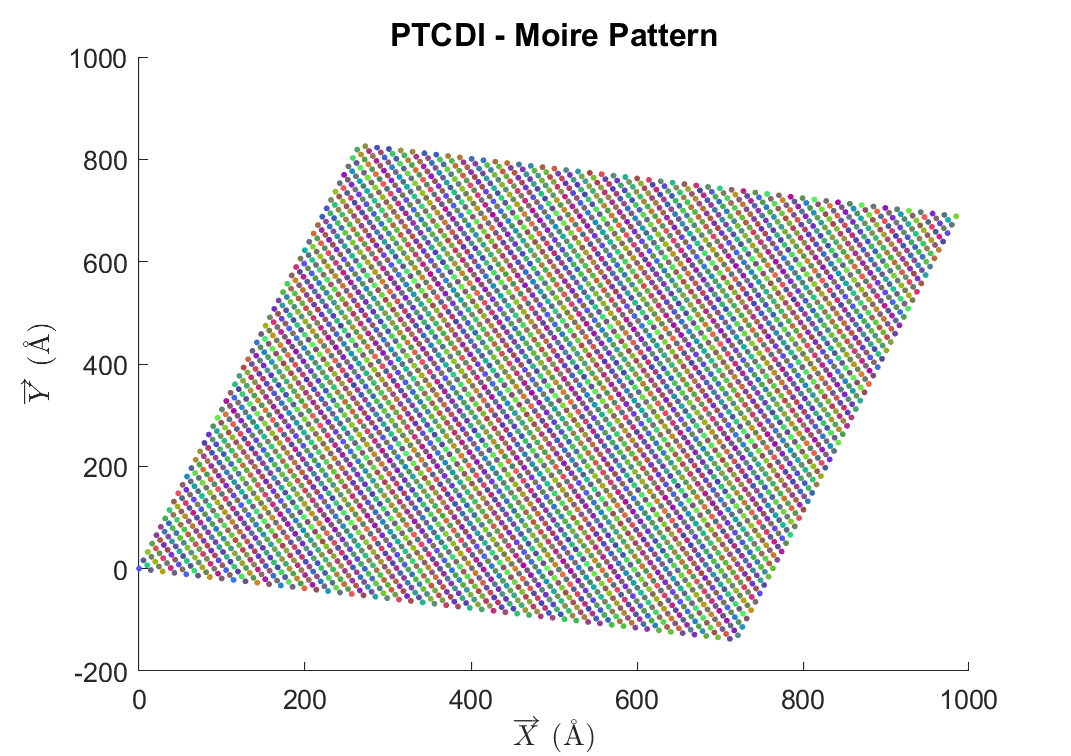
\includegraphics[width = 4 in]{PTCDI-Moire.png}}
\subcaptionbox{\label{fig:PTCDI-UPS}}{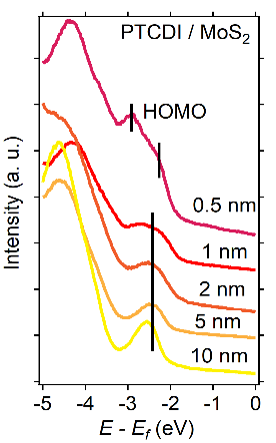
\includegraphics[scale = 1.4]{PTCDI-UPS.png}}
\subcaptionbox{\label{fig:PTCDA-moire}}{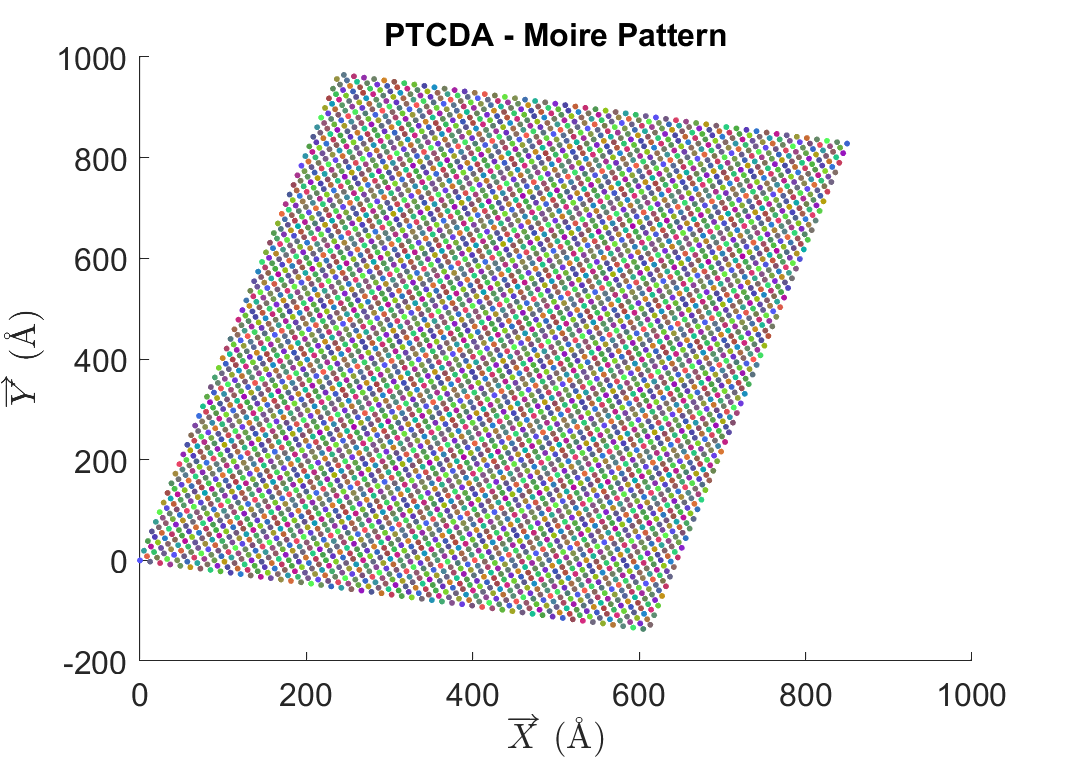
\includegraphics[width = 4 in]{PTCDA-moire.png}}
\subcaptionbox{\label{fig:PTCDA-UPS}}{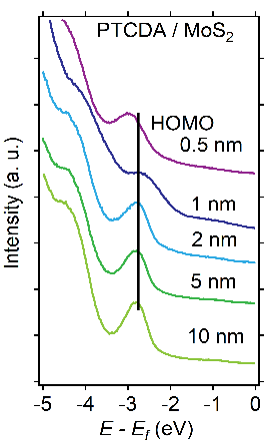
\includegraphics[scale = 1.4]{PTCDA-UPS.png}} 
%\subcaptionbox{\label{fig:PTCDI-LEED}}{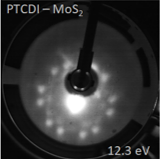
\includegraphics[scale = 0.8]{PTCDI-LEED.png}}
%\subcaptionbox{\label{fig:PTCDA-LEED.png}}{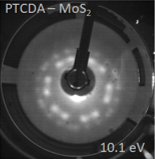
\includegraphics[scale = 0.8]{PTCDA-LEED.png}}
\caption{Simulated moire patterns of (a) PTCDI and (c) PTCDA on MoS$_2$. UPS spectra of (b) PTCDI on ML-MoS$_2$ and (d) PTCDA on ML-MoS$_2$.}\label{fig:Moire}
\end{figure}
Another way to study the nanopatterns in the heterostructures is by looking at their moire patterns. These patterns are naturally formed whenever two crystals having different lattice parameters and/or symmetries are placed on top of each other. Such patterns leads to the modulation of the potential energy landscape near the interface which are reffered to as moire potential. In TMDC heterostructures, the moire potential has been used to control the exciton dynamics and emissive properties of excitons \cite{yuan2020twist,bai2020excitons,seyler2019signatures}. We then went on to study whether such patterns could impact the electronic properties and dynamics of CT-excitons in TMDC / organic heterostructures, which play a significant role in photo-to-electrical conversion yield.

\vspace{7pt}

We simulated the moire patterns in the MoS$_2$/PTCDA and MoS$_2$/PTCDI heterostructures, using their reported lattice parameters and orientations in bulk MoS$_2$ (obtained from the STM measurements \cite{ludwig1994stm}). Figures \ref{fig:PTCDI-moire} and \ref{fig:PTCDA-moire} show the moire patterns from the MoS$_2$/PTCDA and MoS$_2$/PTCDI heterostructures respectively. Each lattice site of the organic crystal is represented by a colored dot. The color of each lattice site is scaled to map its distance from the nearby MoS$_2$ molecule. In ML-MoS$\protect_2$ / PTCDI heterostructure, we observed a regular pattern evolving over the plane with the periodicity of $\sim \SI{50}{\angstrom}$ (Figure \ref{fig:PTCDI-moire}). However, in the case of the ML-MoS$\protect_2$ / PTCDA heterostructure, it is more random and we do not see such a regular pattern evolving over a similar distance (Figure \ref{fig:PTCDA-moire}). To study the potential impacts of such patterns on energy levels near the interface of these heterostructures, we prepared the PTCDA and PTCDI heterostructures on ML-MoS$_2$ through vapor deposition technique inside the UHV chamber and took UPS measurements. The lattice parameters and orientation of organic crystals in the heterostructure were measured with the help of LEED experiments and were in good agreement with the parameters used in our simulation. The results of our measurements are summarized in Table \ref{tab:table1}. UPS spectra in Figure \ref{fig:PTCDI-UPS} shows that the HOMO peak of ML - MoS$_2$ / 0.4 nm PTCDI is split into two peaks with the separation of $\sim$ 0.68 eV which gradually vanishes as the thickness of the film is increased. The vanishing of the split peaks for higher thicknesses can be explained by the fact that the UPS technique being used is very surface sensitive and as the thickness of the film increases the phenomenon occurring at the interface becomes less and less pronounced. As a result, the peaks we see are dominated by the organic molecules on the surface of sample. However, there is no such peak splitting in the case of ML - MoS$_2$ / PTCDA heterostructures. Whether the splitting observed is direct consequence of moire patterns or not remains unclear, and we are looking at their theoretical origins through collaboration.


\begin{table} [H]
\centering
\begin{tabular}{lcc}
\hline
\textbf{Molecule} & \textbf{PTCDA} & \textbf{PTCDI} \\
\hline
a\textsubscript{1} & 12.5 $\pm$ 0.6 \AA & 14.1 $\pm$ 0.6 \AA \\
a\textsubscript{2} & 20.0 $\pm$ 0.2 \AA & 17.1 $\pm$ 0.2 \AA \\
Molecules per unit cell & 2 & 2 \\
$\Gamma = \angle$(a\textsubscript{1},a\textsubscript{2}) & $90^\circ$ $\pm$ $1.9^\circ$ & $85.1^\circ$ $\pm$ $2.2^\circ$ \\
$\Phi = \angle$(A\textsubscript{MoS\textsubscript{2}},a\textsubscript{1}) & $17.9^\circ$  $\pm$ $4.4^\circ$ & $14.1^\circ$ $\pm$ $4.7^\circ$ \\
\hline
\end{tabular}
\caption{Lattice parameters obtained from LEED measurements}
\label{tab:table1}
\end{table}


\section{Future plans}
% It is essential to select donor and acceptor molecules with suitable bandgaps in order to study the exciton dissociation process in type-II heterojunctions. We plan to design and study organic bilayer heterojunctions, bulk heterojunctions and hybrid (TMDC-Organic) heterostructures using different molecules as donor and acceptor. We will focus on non fullerene acceptors like PTCDA, PTCDI and Y6 in our future works since fullerenes are less desired in BHJs due to their high cost, difficulty in chemical modification and unstable device performance \cite{he2011fullerene}. On the other hand, NFAs have been very successful in recent years in achieving higher PCEs for the reasons that are not well understood \cite{lin2015electron}. We plan to use morphologically different donor molecules like PM6 (Polymer), MoS$_2$(TMDC) and SubPc with different morphologies and can tune the E$_{off}$ at the interface.

\subsection{MoS$\protect_2$ / PTCDA and MoS$\protect_2$ / PTCDI heterostructure}
 We intend to further study the nanopatterns and their roles in HOMO splitting, electron delocalization, exciton dynamics, and exciton dissociation at the MoS$_2$ / PTCDI and MoS$_2$ / PTCDA interfaces. These investigations can be carried out by using TR-TPPE measurements. We are also currently collaborating with research groups at KU for transient reflection measurements (TR) and photo luminiscent measurements (PL) on the samples. The PL measurements help us to find the CT-exciton peaks in the MoS$_2$ / PTCDI and MoS$_2$ / PTCDA interfaces. The dynamics of such CT-excitons and their delocalization and dissociation can be studied by TR-TPPE measurements of interfaces with varying thicknesses. These measurements can be cross examined and verified with the help of TR measurements which are not surface sensitive unlike TR-TPPE. The results from these studies could potentially answer very challenging questions such as do moire patterns play a significant role in the exciton dynamics in the organic semiconductors and should that factor be considered while designing interfaces for better efficiencies in organic or hybrid BHJs.

\subsection{MoS$\protect_2$ / SubPc heterostructure}
Different moire patterns can also be produced using same molecules but having different crystal structures. For e.g. in CuPc molecules deposited on MoS$_2$ substrate show two phases, one close-packed and one row-like phase \cite{ludwig1994epitaxy}. Our simulation shows two different moire patterns for these phases (Figure \ref{fig:CuPc Moire}). CuPc molecules belongs to the group of metal pthalocyanines such as ZnPc and SubPc which show polymorphism when grown on substrates through vapor deposition technique. While ZnPc and CuPc are planar molecules, SubPc is a non-planar molecule with three N-fused di-iminoisoindole rings, centered around a boron core (Figure \ref{fig:SubPc molecule}). This non-planar structure can be modified to have different packing orientations, depending on the deposition conditions. In general, the temperature of the substrate affects the molecular orientation of SubPc, which is essential to the carrier transport of the material. Indeed, in SubPc molecules, AFM and SEM measurements have shown different morphologies when grown at different substrate temperatures. In particular, at 120$^\circ$ C SubPc film was found to be dominated by (221) plane orientation which is advantageous for carrier transport (Figure \ref{fig:SubPc Xray}) \cite{chou2012effect}.

\begin{figure}[H]
\centering
\subcaptionbox{\label{fig:close-packed}}{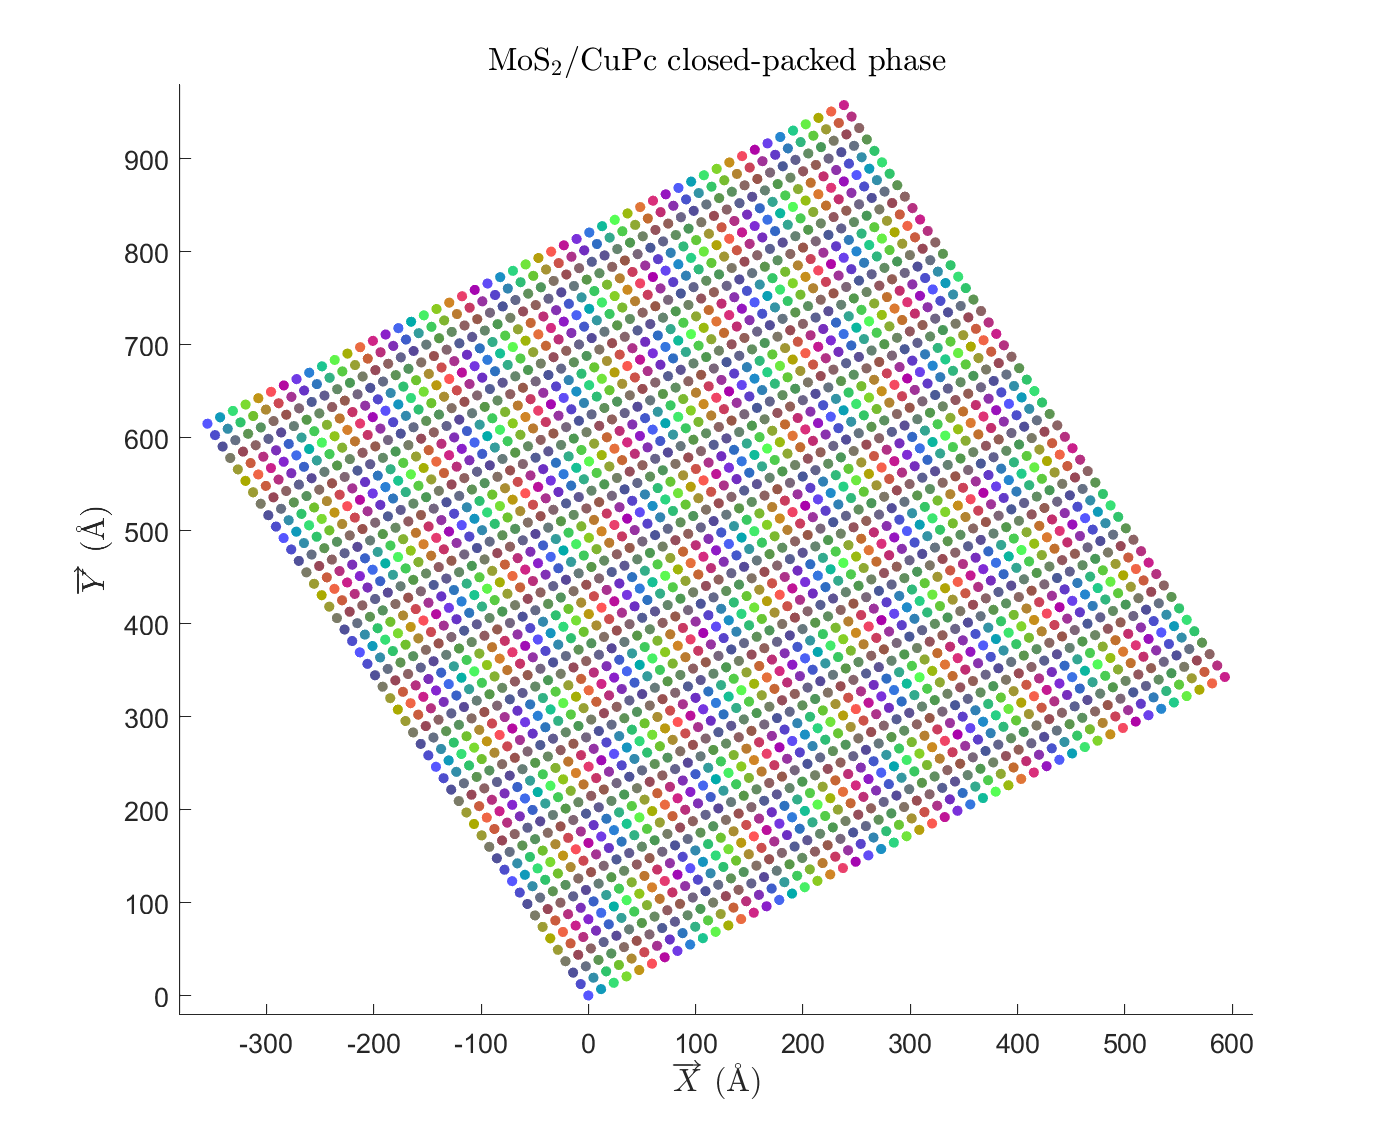
\includegraphics[scale = 0.2]{CuPc hexagon full.png}}\hspace{0pt}
\subcaptionbox{\label{fig:row-like}}{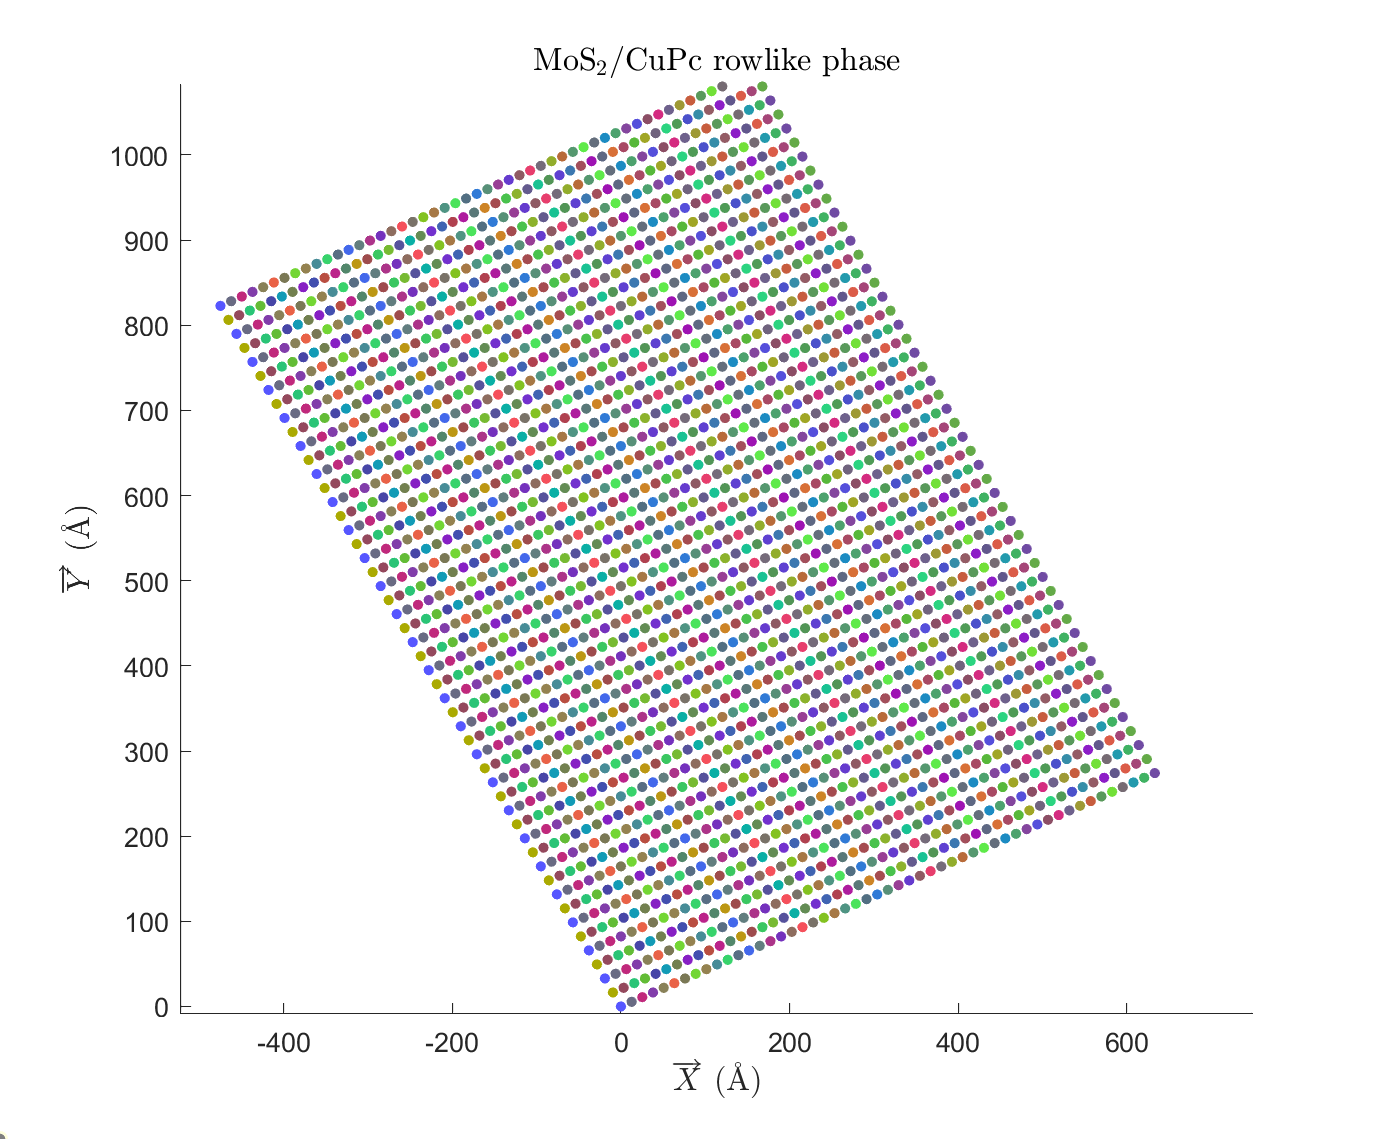
\includegraphics[scale = 0.2]{CuPc rowlike-new-full.png}}
\caption{Simulated moire patterns of MoS$_2$ / CuPc heterostructures in (a) close-packed phase and (b) row-like phase.}\label{fig:CuPc Moire}
\end{figure}


\begin{figure}[H]
\centering
\subcaptionbox{\label{fig:SubPc molecule}}{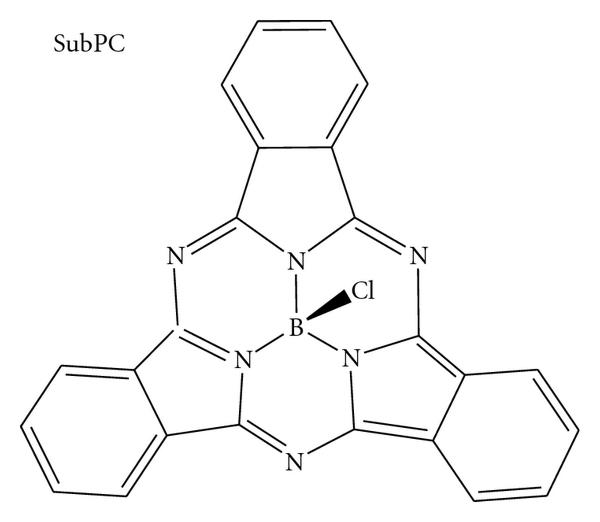
\includegraphics[scale=1]{SubPc molecules.png}}\hspace{10pt}
\subcaptionbox{\label{fig:SubPc Xray}}{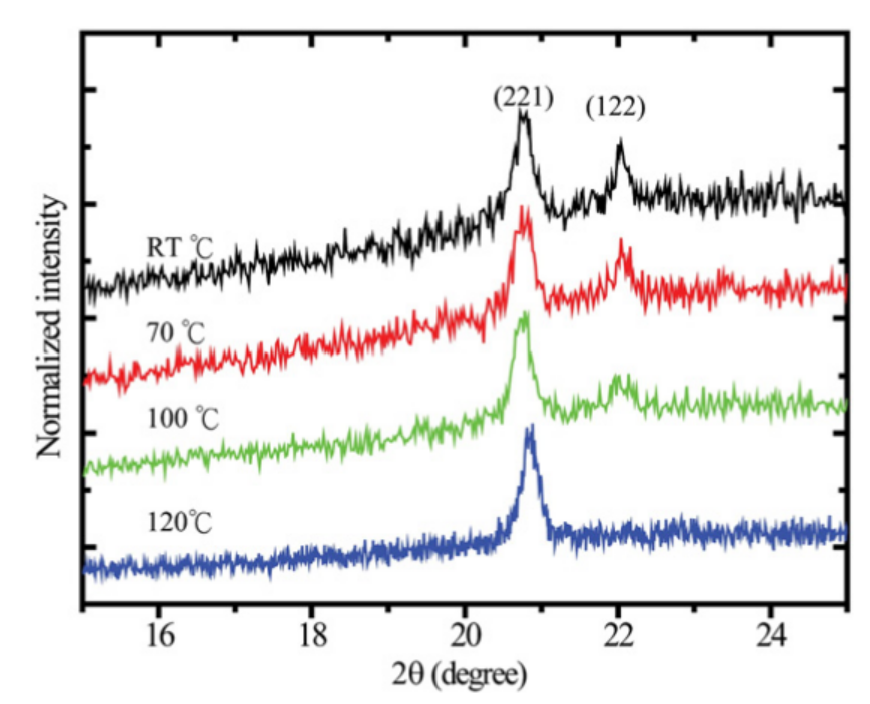
\includegraphics[scale=0.6]{SubPc orientation.png}}
\caption{(a) Molecular structure of SubPc (b) X-ray diffraction data of SubPc at different substrate temperatures \cite{chou2012effect}.}\label{fig:SubPC temp}
\end{figure}
Unlike CuPc molecules, SubPc molecules can be grown with control over their phase on MoS$_2$ molecules at different temperatures. We can closely monitor the crystal structures of SubPc molecules in both phases using LEED measurements. We plan to further investigate the  effects of different crystal structures and morphologies at different substrate temperature on electronic properties and exciton dynamics at the interface using UPS and TR-TPPE experiments. The results of these experiments combined with results from the MoS$\protect_2$ / PTCDA and MoS$_2$ / PTCDI heterostructure could further elucidate the impact of nanopatterns on the device performance.


\subsection{PM6/Y6 heterostructure}
PM6 and Y6 are the organic semiconductors used in champion OSCs with record-breaking efficiencies as donor and acceptor molecules, respectively. We have obtained the Y6 and PM6 from a vendor and the BHJs will be made by using
the spin-coating techniques. BHJ OSCs prepared  by using one-step deposition technique where both donor and acceptor molecules are mixed and spin-coated are known to result in giving a complex photovoltaic  morphology, that depends on  the conditions of blend solution and hence resulting in an undesirable vertical phase separation. We plan to use the sequential deposition technique where we deposit PM6 and Y6 molecules in two steps on the ITO substrate using spin-coating. To make PM6 and Y6 solutions for spin-coating, we will follow the standard protocols reported in the literature. Furthermore, the conductivity of the ITO substrate can be enhanced by spin-coating a layer of PEDOT:PSS and the crystalline texture of Y6 molecules can be improved by using chloronapthalene (CN) as an additive.

To prove our hypothesis on CT exciton heating process, we will study the CS mechanism at the D-A interfaces to demonstrate that the exciton heating process occurs in these BHJs, which can explain their extraordinary efficiencies. By using the TR-TPPE measurements, we further aim to show that, in this interface, exciton heating can minimize the energy loss during the charge separation process.



\section{Summary}
In summary, we hypothesize that due to the collective effect of entropy, electron delocalization and nano-pattern of the NFAs, exciton heating process can occur in certain interfaces containing NFA molecules. We can test this idea by employing UPS and TR-TPPE techiniques to study the dynamical evolution of CT excitons and their dissociation in different heterostructures. By using UPS and TR-TPPE measurements on MoS$_2$/PTCDA, MoS$_2$/PTCDI, and MoS$_2$/ SubPc heterostructures, we can study the role of nanopatterns on electron transfer across the interface, electron delocalization and charge separation. Similarly, UPS and TR-TPPE studies on PM6/Y6 BHJ allows us to directly test if CT exciton heating process is responsible for the record breaking gain in OPV efficiency.

\bibliographystyle{unsrt}
\bibliography{references}

\end{document}
